%\documentclass[9pt,twocolumn]{scrartcl}


\documentclass[9pt]{sigcomm-alternate}

%\usepackage[margin=1in,bottom=1.2in]{geometry}
\usepackage{amsfonts,amssymb,amsmath}
%\usepackage[thmmarks,hyperref,amsthm,amsmath]{ntheorem}
\usepackage{graphicx}
\usepackage[ruled,vlined,commentsnumbered]{algorithm2e}
\usepackage[usenames,dvipsnames]{color}
\usepackage{hyperref}
\usepackage{multirow}
\usepackage{lineno}
\usepackage[shortlabels]{enumitem}
\usepackage[utf8]{inputenc}
\usepackage[OT4]{fontenc}
\usepackage{comment}
\usepackage{fancyhdr}
%\usepackage{tikz-cd}
\usepackage{wrapfig}
%Used Symbols
%c_i = chunk i
%v_i = vm i
%b_t = transfer bandwidth
%b_c = pairwise communication bandwidth
%n = |VMs| = |Chunks|


%Header Extensions Seperation
%Carlo
\newcommand{\VmSlot}{\text{VM slot}}
\newcommand{\VmSlots}{\VmSlot\text{s}}
%\newcommand{\Capacity}{\ensuremath{\textsc{cap}}}
\newcommand{\VM}{\textsc{VM}}
\newcommand{\Problem}{\textsc{DummyName Problem}}
\newcommand{\carlo}[1]{\textcolor{red}{carlo: #1}}
\newcommand{\maciek}[1]{\textcolor{brown}{maciek: #1}}
\newcommand{\stefan}[1]{\textcolor{blue}{stefan: #1}}
\newcommand{\MaFactor}{m}
\newcommand{\Path}{\ensuremath{p}}
\newcommand{\RedundancyFactor}{\ensuremath{r}}

\newcommand{\variab}{\nu}

\newcommand{\Source}{\ensuremath{s^{+}}}
\newcommand{\Sink}{\ensuremath{s^{-}}}

\newcommand{\VmChunkAssignment}{\mu}
\newcommand{\NodeMapping}{\pi}
\newcommand{\ChunkLocation}{\pi}

\newcommand{\ChunkType}{\tau}
\newcommand{\VirtualNodes}{\ensuremath{V}}
\newcommand{\VirtualEdges}{\ensuremath{E_V}}
\newcommand{\VirtualNode}{v}
\newcommand{\VirtualEdge}{e}
\newcommand{\VCSwitch}{\ensuremath{\textsc{center}}}
\newcommand{\SubstrateNodes}{\ensuremath{V_S}}
\newcommand{\SubstrateEdges}{\ensuremath{E_S}}
\newcommand{\SubstrateNode}{\ensuremath{v}}
\newcommand{\SubstrateEdge}{\ensuremath{e}}
\newcommand{\Leaf}{\ensuremath{l}}
\newcommand{\Leaves}{\ensuremath{L}}
\newcommand{\Chunks}{\ensuremath{\textsc{chunks}}}
\newcommand{\aroot}{\emph{root}}

\newcommand{\Opt}{\ensuremath{Opt}}
\newcommand{\Children}{\ensuremath{children}}
%\newcommand{\Cost}{\ensuremath{\textsc{cost}}}

\newcommand{\Uplink}{\ensuremath{\textsc{uplink}}}
\newcommand{\ChunkCount}{\ensuremath{\textsc{cis}}}
\newcommand{\VmCount}{\ensuremath{\textsc{vis}}}
\newcommand{\Right}{\ensuremath{r}}
\newcommand{\InverseAssignment}{\ensuremath{\VmChunkAssignment^{-1}}}

\newcommand{\clauses}{\alpha}
\newcommand{\vars}{\beta}
\newcommand{\variables}{\beta}
\newcommand{\achunk}{\ensuremath{c}}
\newcommand{\Chunk}{\ensuremath{c}}
\newcommand{\capa}{\emph{cap}}
\newcommand{\capacity}{\emph{cap}}
\newcommand{\Distance}{\emph{\textsc{dist}}}
\newcommand{\dist}{\emph{dist}}
\newcommand{\CostPerChunk}{\emph{cost}}


\newcommand{\VC}{\textsc{VC}}
\newcommand{\CC}{\textsc{NI}}

\newcommand{\VE}{\textsc{VE}}
\newcommand{\FP}{\textsc{FP}}
\newcommand{\RS}{\textsc{RS}}
\newcommand{\BW}{\textsc{BW}}
\newcommand{\MA}{\textsc{MA}}
\newcommand{\Cost}{\textsc{F}}

\newcommand{\MatchCost}{\textsc{MCost}}
\newcommand{\chunkOf}{\textsc{chunkOf}}



\newtheorem{defn}{Definition}
\newtheorem{obs}{Observation}

%Maciek

\newcommand{\Bandwidth}{\ensuremath{bw}}
\newcommand{\Tree}{\ensuremath{T}}
\newcommand{\CostTrans}{\ensuremath{b_1}}
\newcommand{\CostCom}{\ensuremath{b_2}}
\newcommand{\Vms}{\ensuremath{n_V}}
\newcommand{\TSC}{\textsc{3-SC}}
\newcommand{\TDM}{\textsc{3-DM}}
\newcommand{\TSAT}{\textsc{3-Sat}}
\newcommand{\NSAT}{\textsc{Sat}}
\newcommand{\SAT}{\textsc{Sat}}
\newcommand{\ZSAT}{\textsc{2-Sat}}


\newcommand{\Formula}{\ensuremath{\Psi}}
\newcommand{\Clauses}{\ensuremath{Cl(\Formula)}}
\newcommand{\NClauses}{\ensuremath{c}}
\newcommand{\Vars}{\ensuremath{Var(\Formula)}}
\newcommand{\NVars}{\ensuremath{|\Vars|}}
\newcommand{\ChunkTypes}{\ensuremath{ch}}
\newcommand{\Thr}{\ensuremath{Th}}
\newcommand{\VCB}{\ensuremath{VCB}}
\newcommand{\VCNB}{\ensuremath{VCNB}}
\newcommand{\varx}{\ensuremath{x}}
\newcommand{\positive}{\ensuremath{positive}}
\newcommand{\negative}{\ensuremath{negative}}
\newcommand{\Val}{\ensuremath{Val}}
\newcommand{\Sol}{\ensuremath{SOL}}



\definecolor{blueLink}{rgb}{0,0.2,0.8}
\hypersetup{colorlinks,linkcolor=blueLink,urlcolor=blueLink,citecolor=blueLink}
\newcommand{\lref}[2][]{\hyperref[#2]{#1~\ref*{#2}}}



%%%%%%%%%%%%%%%%%%%%%%%%%%%%%%%%%%%%%%%%%%%%%%%%%%%%%%%%%%%%%
% GENERAL STYLE MACROS
%%%%%%%%%%%%%%%%%%%%%%%%%%%%%%%%%%%%%%%%%%%%%%%%%%%%%%%%%%%%%

\newcommand{\etal}{{\it et~al.\ }}
\newcommand{\myparagraph}[1]{{\smallskip\noindent{\bf #1}}}
\newcommand{\mycase}[1]{{\underline{Case~#1}:}}

%%%%%%%%%%%%%%%%%%%%%%%%%%%%%%%%%%%%%%%%%%%%%%%%%%%%%%%%%%%%
% THEOREMS AND SUCH
%%%%%%%%%%%%%%%%%%%%%%%%%%%%%%%%%%%%%%%%%%%%%%%%%%%%%%%%%%%%%

\newtheorem{theorem}{Theorem}
\newtheorem{corollary}[theorem]{Corollary}
\newtheorem{lemma}[theorem]{Lemma}
\newtheorem{claim}[theorem]{Claim}
\newtheorem{fact}{Fact}

%%%%%%%%%%%%%%%%%%%%%%%%%%%%%%%%%%%%%%%%%%%%%%%%%%%%%%%%%%%%%
% USEFUL LETTERS
%%%%%%%%%%%%%%%%%%%%%%%%%%%%%%%%%%%%%%%%%%%%%%%%%%%%%%%%%%%%%

\DeclareMathOperator{\polylog}{polylog}
\newcommand{\emdash}{\hspace{1mm}---\hspace{1mm}}
\newcommand{\e}{\mathrm{e}}
\renewcommand{\O}{\mathcal{O}}
\renewcommand{\Pr}{\mathbf{Pr}}
\newcommand{\E}{\mathbf{E}}
\newcommand{\NAT}{\mathbb{N}}
\newcommand{\REAL}{\mathbb{R}}

%%%%%%%%%%%%%%%%%%%%%%%%%%%%%%%%%%%%%%%%%%%%%%%%%%%%%%%%%%%%%
% PARENTHESES ETC
%%%%%%%%%%%%%%%%%%%%%%%%%%%%%%%%%%%%%%%%%%%%%%%%%%%%%%%%%%%%%

\newcommand{\ceiling}[1]{\left\lceil #1 \right\rceil}
\newcommand{\floor}[1]{\left\lfloor #1 \right\rfloor}
\newcommand{\braced}[1]{{\left\{#1\right\}}}
\newcommand{\bigbrackd}[1]{{\big[#1\big]}}
\newcommand{\brackd}[1]{{\left[#1\right]}}
\newcommand{\parend}[1]{{\left(#1\right)}}

%%%%%%%%%%%%%%%%%%%%%%%%%%%%%%%%%%%%%%%%%%%%%%%%%%%%%%%%%%%%%
% FRACTIONS
%%%%%%%%%%%%%%%%%%%%%%%%%%%%%%%%%%%%%%%%%%%%%%%%%%%%%%%%%%%%%

\newcommand{\half}{\frac{1}{2}}
\newcommand{\onehalf}{\frac{1}{2}}
\newcommand{\onethird}{\frac{1}{3}}
\newcommand{\twothirds}{{\textstyle\frac{2}{3}}}
\newcommand{\fourthirds}{{\textstyle\frac{4}{3}}}
\newcommand{\fivethirds}{{\textstyle\frac{5}{3}}}
\newcommand{\threefourths}{{\textstyle\frac{3}{4}}}

%%%%%%%%%%%%%%%%%%%%%%%%%%%%%%%%%%%%%%%%%%%%%%%%%%%%%%%%%%%%%
% ALGORITHM NAMES, ETC
%%%%%%%%%%%%%%%%%%%%%%%%%%%%%%%%%%%%%%%%%%%%%%%%%%%%%%%%%%%%%

\newcommand{\ALG}{\textsc{Alg}}
\newcommand{\OPT}{\textsc{Opt}}
\newcommand{\DET}{\textsc{Det}}
\newcommand{\RAND}{\textsc{Rand}}

%%%%%%%%%%%%%%%%%%%%%%%%%%%%%%%%%%%%%%%%%%%%%%%%%%%%%%%%%%%%%
% PSEUDOCODE
%%%%%%%%%%%%%%%%%%%%%%%%%%%%%%%%%%%%%%%%%%%%%%%%%%%%%%%%%%%%%

\newcommand{\IF}    {{\bf if }}
\newcommand{\THEN}  {{\bf then }} 
\newcommand{\FOR}   {{\bf for }}
\newcommand{\EACH}  {{\bf each }} 
\newcommand{\DO}  {{\bf do }} 

%%%%%%%%%%%%%%%%%%%%%%%%%%%%%%%%%%%%%%%%%%%%%%%%%%%%%%%%%%%%%
% EDITORIAL MACROS
%%%%%%%%%%%%%%%%%%%%%%%%%%%%%%%%%%%%%%%%%%%%%%%%%%%%%%%%%%%%%

\definecolor{brown}{rgb}{0.4,0,0} 
\definecolor{purple}{rgb}{0.2,0,0.6}
\definecolor{hotpink}{rgb}{1,0.4,0.7}
\newcommand{\marginnote}[1]{\marginpar{\scriptsize{\begin{flushleft}#1\end{flushleft}}}}
\newcommand{\todo}[1]{\noindent\colorbox{red}{todo: #1}} 
\newcommand{\marcin}[1]{\color{red} Marcin: #1\color{black}}



\title{A Note on Virtual Cluster Embedding with Data Locality}

\title{Embedding Algorithms for Virtual Clusters with Data Locality and Replica Selection}

\title{Embedding Virtual Clusters with Data Locality and Replica Selection\\{\Large Real Algorithms for Virtual Environments}}

\title{Data Locality and Replica Aware Virtual Cluster Embeddings}
%\\{\Large Real Algorithms for Virtual Environments}}


\author{Paolo Costa$^1$, Carlo Fuerst$^2$, Maciej Pacut$^3$, Stefan Schmid$^4$\\
{\small $^1$ MSR, UK; $^2$ TU Berlin, Germany; $^3$ University of Wroclaw, Poland; $^4$ TU Berlin \& T-Labs, Germany}}

\begin{document}

\maketitle


\begin{abstract}
Virtualized datacenters offer great flexibilities in terms of resource allocation. In particular, by
decoupling applications from the constraints of the underlying physical infrastructure, virtualization
supports an optimized mapping of virtual machines as well as their interconnecting network
% (the so-called \emph{virtual cluster})
to their
physical counterparts: essentially a graph embedding problem.

However, existing algorithms
in the literature often ignore a crucial dimension of the embedding problem, namely \emph{data locality}:
the input to a cloud application such as MapReduce is typically stored in a distributed,
and sometimes redundant, file system. Since moving
data is costly, an embedding algorithm should be data locality aware,
and allocate computational resources close to the data; in case of redundant storage, the algorithm should also optimize the \emph{replica selection}.

This paper initiates the algorithmic study of data locality aware virtual cluster embeddings
% for
%the widely used (fat-)tree like
on datacenter topologies.
In particular, we
show that
despite the multiple degrees of freedom in terms of embedding, replica selection and assignment,
many problems can be
solved efficiently\maciek{Passive voice - consider rewrite.}
. However, we also show the limitations of such optimizations,
by presenting several NP-hardness proofs; interestingly,
our hardness results also hold in uncapacitated networks and in networks of small diameter.
\end{abstract}

%\begin{comment}
%we should maybe give the main algorithms a name; we should talk about the case where the number of machines is not a perfect multiple;
%\end{comment}

%\section*{TODOs}%
%
%determine all runtimes (check related work for flow and match!), make float-figures, finish appendix, order properties in the same way always (the order we had in the %model!)

%%%%%%%%%%%%%%%%%%%%%%%%%%%%%%%%%%%%%
\section{Introduction}

%Server virtualization has revamped the server business over the last years,
%and has radically changed the way we think about resource allocation:
%today, almost arbitrary computational resources can be allocated on demand.
%Moreover, the virtualization trend now started to spill over to the network:
%batch-processing applications such as MapReduce often generate significant
%network traffic (namely during the so-called shuffle phase)~\cite{amazonbw},
%and in order to avoid interference in the underlying physical network and in order to provide a predictable
%application performance, it is important to provide performance isolation and bandwidth guarantees
%for the virtual network connecting the virtual machines.~\cite{talk-about}

Distributed cloud applications, such as batch-processing applications or scale-out databases, generate a significant amount of network traffic.~\cite{talk-about}
For instance, MapReduce applications consist of a network intensive shuffle phase,
where data is transferred from the mappers to the reducers.
In order to ensure a predictable application performance, especially in shared cloud environments,
it is hence important to provide isolation and bandwidth guarantees between the virtual machines~\cite{amazonbw},
e.g., by making explicit network reservations.~\cite{oktopus}
Accordingly, modern batch-processing applications provide the abstraction of entire \emph{virtual networks}~\cite{talk-about},
defining both the virtual machines
as well as their interconnecting network. The most prominent virtual network abstraction is the \emph{virtual cluster}~\cite{oktopus,proteus}.

Virtualized datacenters
offer great flexibilities on where these virtual networks
can be instantiated or \emph{embedded}\maciek{Passive voice - consider rewrite.}
.
In order to maximize the resource utilization in the datacenter, it is in principle desirable to
map the virtual machines of a given virtual network as close as possible
in the underlying physical network, as this minimizes communication costs (respectively, bandwidth reservations).~\cite{oktopus,proteus}

However, existing systems often ignore a crucial dimension of the virtual network embedding problem: 
the fact that the input data for a cloud application is typically distributed across different servers and stored in a distributed file system~\cite{hdfs}.
In order to properly minimize
communication costs, an embedding algorithm should hence also be \emph{data locality aware},
and allocate (or \emph{embed}) computational resources close to the to be processed data.
Moreover, in case of redundant storage (batch processing
applications often provide a 3-fold redundancy~\cite{hdfs}), an algorithm should also be aware of, and exploit, \emph{replica selection}
flexibilities.

\subsection{Our Contributions}

This paper initiates the study of data-locality and replica aware virtual network embedding problems in datacenters.
In particular, we decompose the optimization problem into different fundamental aspects, such as
chunk assignment, replica selection, or flexible virtual machine placement, and answer questions such as:
\begin{enumerate}
\item Which chunks to assign to which virtual machine?

\item How to efficiently select replicas?

\item How to efficiently embed virtual machines and their inter-connecting network?

\item Can the chunk assignment, replica selection and virtual machine embedding problems be jointly optimized, in polynomial time?
\end{enumerate}

We draw a complete picture of the problem space: We show that
even problem variants exhibiting multiple degrees of freedom in terms of
replica selection and embedding,
can be solved optimally in polynomial time, and present several efficient
algorithms accordingly\maciek{Passive voice - consider rewrite.}
. However, we also prove limitations in terms of
computational tractability, by providing reductions from 3-D matching
and Boolean satisfiability ($\SAT$). Interestingly,
while it is well-known that (unsplittable) multi-commodity flow
problems are NP-hard in capacitated networks, our hardness results also hold in \emph{uncapacitated}
networks; moreover, we show that NP-hard problems already arise in small-diameter networks (as they are
widely used today~\cite{fattree}),
and even if the number of replicas is bounded by two.


\subsection{Organization}

The remainder of this paper is organized as follows.
Section~\ref{sec:model} introduces our formal model in detail.
Algorithms are presented in Section~\ref{sec:poly} and
hardness results are presented in Section~\ref{sec:np}.
After discussing related work in Section~\ref{sec:relwork},
we conclude our work in Section~\ref{sec:conclusion}.
Some technical details as well as additional hardness results
appear in the Appendix.

\section{Model}\label{sec:model}

To get started, let us first introduce our model as well as its constituting parts \emph{formally}.
For the sake of clarity, we defer the discussion of the practical background and motivation
to the end of this section. Figure~\ref{fig:overview} gives an overview of our model.

\begin{figure}[t]
\centering
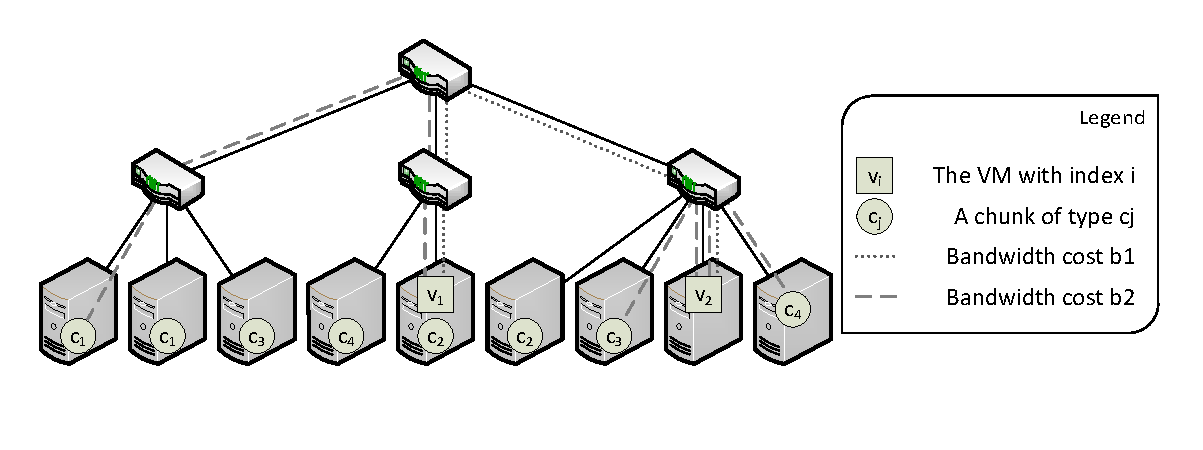
\includegraphics[width=0.99\columnwidth]{figs/overview-fig.pdf}
\caption{Overview: a 9-server (fat-tree) datacenter storing $\tau=4$ different chunk
types $\{c_1,\ldots,c_4\}$ (depicted as \emph{circles}). The chunk replicas need to be selected and assigned to the two
 virtual machines $v_1$ and $v_2$; the virtual machines are depicted as \emph{squares}, and
 the network connecting them to chunks is \emph{dashed}. In addition, the virtual machines are inter-connected among
 each other (\emph{dotted}). The objective of the embedding problem is to minimize the overall bandwidth allocation
 (sum of \emph{dashed} and \emph{dotted} lines).\maciek{Consider moving legend to caption and scale the network figure up.}}
\label{fig:overview}
\end{figure}


%\textbf{Fundamental Parts.}

\subsection{Fundamental Parts}

Our model consists of three fundamental parts: (1) the substrate network (the servers
and the connecting physical network),
(2) the to be processed input (the data chunks), and
(3) the virtual network (the virtual machines and the logical network connecting the machines to each other
as well as to the data).

\textbf{\emph{The Substrate Network.}} The substrate network (also known as the \emph{host graph}) represents the physical resources:
a set $S$ of $n_S=|S|$ servers interconnected by a network consisting of a set $R$ of routers (or switches)
and a set $E$ of (symmetric) links; we will often refer to the elements in $S$ and $R$
as the \emph{vertices}. We will assume that the inter-connecting network forms an (arbitrary, not necessarily balanced
or regular) tree,
where the servers are located at the tree leaves.
Each server $s\in S$ can host a certain number
of virtual machines (available server capacity $\capacity(s)$), and each link $e\in E$ has a certain bandwidth
capacity $\capacity(e)$.

\textbf{\emph{The Input Data.}} The to be processed data constitutes the input to the batch-processing application.
The data is stored in a distributed manner; this spatial distribution is given and not subject to optimization.
The input data consists of $\tau$ different \emph{chunk types} $\{\achunk_1, \ldots, \achunk_{\ChunkType}\}$,
where each chunk type $\achunk_i$ can have $r_i\geq 1$ instances (or replicas) $\{\achunk_{i}^{(1)},\ldots, \achunk_{i}^{(r_i)}\}$,
 stored at different servers. A single server may host multiple chunks.
%Concretely, for each of the $r\cdot k$ replicas $\achunk_{i}^{(j)}$.
%, we will denote by $\pi(\achunk_{i}^{(j)})$ at
%which server it is stored \maciek{Do we use $\pi$ anywhere else in paper?}.
It is sufficient to process one replica, and we will sometimes refer to this
replica as the \emph{active} (or selected) replica.

\textbf{\emph{The Virtual Network.}} The virtual network consists of a set $\VirtualNodes$ of $n_V=|\VirtualNodes|$ virtual machines,
henceforth often simply called \emph{nodes}.
Each node $v \in \VirtualNodes$ can be placed (or, synonymously, \emph{embedded}) on a server; this placement can be subject
to optimization\maciek{Passive voice - consider rewrite.}
.
Depending on the available capacity $\capacity(s)$ of server $s$, multiple nodes may be hosted on $s$.
We will denote the server $s$ hosting node $v$ by $\pi(v)=s$.
Since these nodes process the input data, they need to be assigned and connected to the
chunks. Concretely, for each chunk type $\achunk_i$, \maciek{(exactly one)} one replica $\achunk_{i}^{(j)}$ must be processed by exactly one node $v$;
which replica $\achunk_{i}^{(k)}$ is chosen is subject to optimization, and 
we will denote by $\mu$ the assignment of nodes to chunks.
%We will typically assume that there are $\MaFactor\geq 1$ times more chunk types to be processed than there are nodes,
%where $\MaFactor$ is an integer;
%We will keep the model general, and consider both the case where there are more chunk types
%than virtual machines (requiring the assignment of multiple chunks per nodes) and the case
%where there are less chunks than virtual machines. (See below for motivations for the different scenarios.)
%each node needs to process the same number of chunks.

In order to ensure a predictable application performance, both the connection to the chunks
as well as the interconnection between the nodes may have to ensure certain
minimal bandwidth guarantees; we will refer to the first type of virtual network as the \emph{(chunk) access
network}, and to the second type of virtual network as the \emph{(node) inter-connect}; the latter 
is modeled as a complete network (a \emph{clique}). Concretely, we assume that an  active chunk
is connected to its node at a minimal (guaranteed) bandwidth $\CostTrans$, and a node is connected to any other node
at minimal (guaranteed) bandwidth $\CostCom$.

%\stefan{TODO: clarify whether there can be multiple chunks and or nodes per server}

%\textbf{Optimization Objective.}

\subsection{Optimization Objective}

Our goal is to develop algorithms which minimize
the \emph{resource footprint}: the guaranteed bandwidth allocation (or synonymously: \emph{reservation}) on all links of the given embedding; note that
only the resource allocation at the links but not at the servers depends on the replica selection or embedding. Thus,
we on the one hand aim to embed the nodes in a locality-aware manner, close to the input data
(the chunks), but at the same time also aim to embed the nodes as close as possible to
each other.

Formally, let $\dist(v,\achunk)$ denote the distance (in the underlying physical network $\Tree$) between a node $v$ and
its assigned (active) chunk replica $\achunk$, and let $\dist(v_1,v_2)$ denote the distance between the two nodes $v_1$ and $v_2$.
We define the \emph{footprint} $\Cost(v)$ of a node $v$ as follows:
$$
\Cost(v) = \sum_{\achunk\in \mu(v)} \CostTrans \cdot \dist(v,\achunk) \underbrace{+ \frac{1}{2} \cdot \sum_{v' \in \VirtualNodes\setminus\{v\}} \CostCom \cdot \dist(v,v')}_{\text{only for inter-connect}},
$$
\noindent where $\mu(v)$ is the set of chunks assigned to $v$. Our goal is to minimize the overall footprint
$\Cost=\sum_{v\in V} \Cost(v)$. Recall Figure~\ref{fig:overview}.

%\textbf{Problem Decomposition.}

\subsection{Problem Decomposition}

In order to chart the landscape of the tractability and intractability of different
problem variants, we decompose our problem into its fundamental aspects, namely replica selection
($\RS$), multiple chunk assignment ($\MA$), flexible node placement ($\FP$), node interconnect ($\CC$),
and bandwidth constraints ($\BW$), as described in the following.
In this paper, we will consider all possible 32 problem variants, where each of these five aspects
can either be enabled or disabled.

\textbf{\emph{Replica Selection ($\RS$).}} The first fundamental problem is replica selection:
if the input data is stored redundantly, the algorithm has the freedom to choose a replica
for each chunk type, and assign it to a virtual machine (i.e., \emph{node}).
% Note that this
%selection or ``matching problem'' is non-trivial, even if the locations of the virtual machines
%are already given \maciek{it is trivial in locations are not given}.
In the following, we will refer to a scenario
with redundant chunks by $\RS$; in the $\RS$-only scenario, the number of chunk types
is equal to the number of nodes. Otherwise, we will add the $+\MA$ property discussed next.

\textbf{\emph{Multiple Assignment ($\MA$).}}
If the number of chunk types $\tau$ is larger than the number of nodes,
each node needs to be assigned multiple chunks. We will refer to such a scenario by $\MA$,
and will denote the number of chunks per node by the integer value $\MaFactor = \tau / n_V$.

%Note that in a scenario with only $\MA$ but without $\RS$, chunk types are not redundant.

\textbf{\emph{Flexible Placement ($\FP$).}} The third fundamental degree of freedom, besides replica selection and assignment,
regards the flexibility in the placement (or synonymously: \emph{embedding}) of nodes on physical servers.
We will refer to this aspect by $\FP$. (Recall that each server $s$ can host $\capa(s)$ nodes.)

%\maciek{Here we would like to
%  introduce hosting multiple VMs in one leaf. How do we do that - by
%  setting global upper bound on number of VMs per leaf - or by
%  per-leaf constant? We also need to update NP-hardness proofs to set
%  those numbers to 1 and to modify the dynamic program's base case.}

\textbf{\emph{Node Interconnect ($\CC$).}} We distinguish between scenarios where bandwidth needs to be reserved
both from each node to its assigned chunks as well as to the other nodes
(i.e., $\CostTrans>0$ and $\CostCom>0$), and
 scenarios where only the (chunk) access network requires bandwidth reservation (i.e., $\CostTrans>0$ and $\CostCom=0$).
 We will refer to the former scenario
where bandwidth needs to be reserved also for the inter-connect, by $\CC$.
We also note that the case $\CostTrans=0$ and $\CostCom>0$ has been studied in prior work~\cite{oktopus,talk-about,proteus},
and refer the reader to our related work section.


\textbf{\emph{Bandwidth Capacities ($\BW$).}}
We distinguish between an uncapacitated and a capacitated scenario where the links
of the substrate network come with bandwidth
constraints, and will refer to the bandwidth-constrained version by $\BW$; the capacity of servers
(the number of nodes which can be hosted concurrently) is always limited.
Note that capacity constraints introduce infeasible problem instances, where it is impossible to
allocate sufficient resources to satisfy an embedding request.
%; in this case, we will say that the
%resource footprint is \emph{infinite}. \maciek{I do not like defining
%  value of footprint of infeasible instance. What is the motivation
%  for that?}

%\textbf{Remark on Practical Motivation.}

\subsection{Practical Motivation}\label{ssec:practice}

We conclude our model discussion by providing the necessary practical background and motivation.
Our model is motivated by batch-processing applications such as MapReduce.
Such applications use multiple nodes to
process data, initially often redundantly stored in a distributed file system implemented
by multiple servers.~\cite{mapreduce}
The standard datacenter topologies today are (multi-rooted) fat-tree resp.~\emph{Clos} topologies,~\cite{fattree,vl2}
hierarchical networks  recursively made of sub-trees at each level; this motivates our
focus on tree-like substrate networks where servers are located at the
tree leaves; note however that our topologies do not have to be balanced. In particular, given the amount of multiplexing over the mesh of links
and the availability of multi-path routing protocol, e.g.~ECMP, the redundant
links can be considered as a single aggregate link for bandwidth
reservations. This is consistent with similar assumptions made in
previous work~\cite{oktopus,proteus}.

During execution, batch-processing applications typically cycle through different phases,
most prominently, a mapping phase and a reducing phase; between the two phases,
a shuffling operation is performed, a phase where the results from the mappers
are communicated to the reducers. Since the shuffling phase can constitute a
non-negligible part of the overall runtime~\cite{orchestra},
and since concurrent network transmissions can introduce interference and
performance unpredictability~\cite{amazonbw}, it is important
to provide explicit minimal bandwidth guarantees.~\cite{talk-about}
In particular, our inter-connect (the virtual network connecting the virtual machines)
is motivated by the popular virtual cluster abstraction.~\cite{oktopus,talk-about,proteus}
In this paper, we extend this model with a notion of data-locality.
In particular, we distinguish between the bandwidth needed between assigned chunk
and node ($\CostTrans$) and the bandwidth needed between
two nodes ($\CostCom$); in practice, for applications with a large
``mapping ratio'' where the mapping phase already reduces the data size significantly,
it may hold that $\CostCom\ll\CostTrans$. 
%Finally, note that it is frequently assumed
%that the nodes implementing the mapper functionality also implement the reducer functionality,
%and vice versa.
% however, it can also make sense to have more mappers or more reducers for
%certain applications.

%%%%%%%%%%%%%%%%%%%%%%%%%%%%%%%%%%%%%
\section{Polynomial-Time Algorithms}\label{sec:poly}

\maciek{Make a summary of runtimes - either here or in the conclusion of the section. Instead of making a summary table of runtimes, we can put a sentence in introduction to algorithm section: (something like this) We managed to obtain runtime: (1) in matching-based approach O(...) (2) in flow-based approach O(...) (3) in dynamic programming-based approach O(...). }


Despite the various degrees of freedom in terms of embedding and replica selection,
 many problem variants can be solved efficiently\maciek{Passive voice - consider rewrite.}
.
 This section introduces three general techniques to solve different problem variants,
 which can roughly be categorized into
 \emph{flow} (Section~\ref{ssec:flow}), \emph{matching} (Section~\ref{ssec:match}) and \emph{dynamic programming}
 (Section~\ref{ssec:dyn}) approaches.
 As we will see, several problems variants can be solved in multiple ways\maciek{Passive voice - consider rewrite.}
 (differing in their runtimes),
 and in each approach, we will summarize the solvable problem variants using a \emph{Venn diagram}.

First, let us make a simplifying observation:
\begin{obs}\label{obs:nofp}
In problems without flexible placement ($\FP$),
the bandwidth required
for the inter-connect network ($\CC$) can generally be allocated \emph{upfront}, as it
does not depend on the replica
selection and assignment.
Accordingly, problem variant $\RS+\MA+\CC +\BW$ (as well as all its subproblems)
can be reduced to $\RS+\MA+\BW$ (resp.~its subproblems)\maciek{Passive voice - consider rewrite.}
.
\end{obs}

\subsection{Flow Algorithms ($\RS+\MA+\CC+\BW$)}\label{ssec:flow}

\begin{wrapfigure}{r}{0.5\columnwidth}
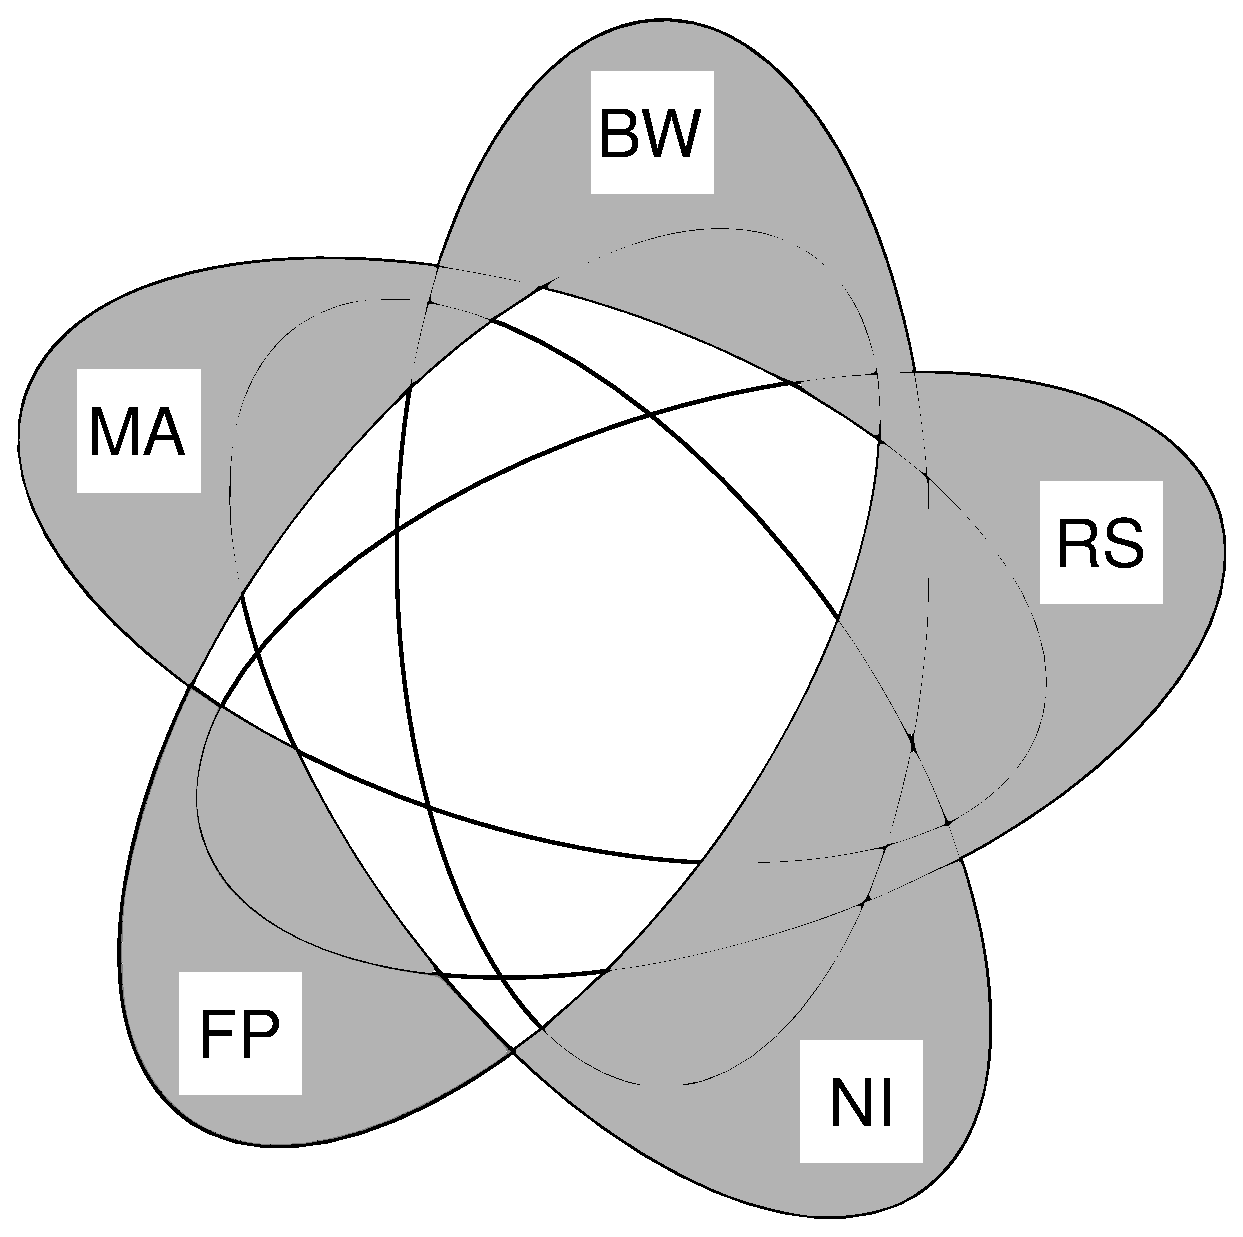
\includegraphics[width=0.48\columnwidth]{figs/venn_flow.pdf}
\caption{Variants solved by flow approach.}
\label{fig:venn_flow}
\end{wrapfigure}

We first present an algorithm to solve the $\RS+\MA+\CC+\BW$ problem.
Recall that in this problem variant,
we are given a set of redundant chunks ($\RS$) and a set of nodes
(the \emph{nodes})
at fixed locations (no $\FP$). The number of chunk types is larger than the number
of nodes ($\MA$), and each node needs to be connected
to its selected chunks as well as to other nodes ($\CC$), while respecting
capacity constraints ($\BW$).
Our goal is to minimize the resource footprint $\Cost$, consisting
of the bandwidth reservations in the (chunk) access network and the (node)
inter-connect.
As we will see in the following, a flow approach can be used to solve this
problem variant\maciek{Passive voice - consider rewrite.}
.

%\maciek{We do not need any assumption about bandwidth. If we do not
%  have integrality, we round down every bandwidth. If we do not have
%  multiplicity of $\CostTrans$, we round to highest $\CostTrans \cdot
%  k$. We can deal with mixing $\CostTrans$ and $\CostCom$ by first
%  decreasing bandwidth by (constant) cost of communication, and then
%  rounding down.}

%We allow an instance to have multiple nodes in single leaf.

\textbf{Construction of Artificial Graph.}
In order to solve the $\RS+\MA+\CC+\BW$ problem,
we first remove the $\CC$ property using Observation~\ref{obs:nofp}.
We then construct
an artificial graph $\Tree^*$, extending the substrate network $\Tree$ and
normalizing bandwidth capacities, as follows. For $\Tree^*$,
we normalize the bandwidth of $\Tree$ to integer multiples of $\CostTrans$,
i.e., for each link $e\in E(\Tree)$, we set its new
capacity in $\Tree^*$ to $\lfloor\capacity(e)/\CostTrans\rfloor$.
%\maciek{I do not understand the floor here. I strongly suggest setting
%$\CostTrans$ to $1$ in the model}
After this normalization, we extend the topology $\Tree$ by
introducing an artificial vertex for each chunk type. These artificial
vertices are connected to each leaf (i.e., server) in $\Tree$ where a replica
 of the respective chunk type is located,
connecting the replica of the respective chunk type by a link of capacity $1$. In
addition, we create a
\emph{super-source} $\Source$, and connect it to each of the artificial chunk
type vertices (with a link of capacity 1). Moreover, we create an artificial \emph{super-sink} $\Sink$ and
connect it to every leaf containing at least one node; the link capacity represents
the number of nodes $x$ hosted on this server, times the multi-assignment factor
$\MaFactor$:
$x \cdot \MaFactor$.
We additionally assign the following costs to edges of $\Tree^*$:
every edge of the original substrate network costs one unit, and all other edges
cost nothing.

%Recall that $\RS+\CC+\MA+\BW$ boils down to
%$\RS+\MA+\BW$ in the absence of $\FP$
The $\RS+\MA+\BW$ problem can now be solved by computing
a \emph{Min-Cost-Max-Flow} solution between super-source $\Source$ and super-sink $\Sink$ on the artificial graph $\Tree^*$.

\textbf{Example.} Figure~\ref{fig:flow_construction} shows an example of the extended substrate
network $\Tree^*$: The source $\Source$ is connected to the two leaves, which host the
nodes. The artificial nodes are depicted below the leaves, are labeled with
their respective chunk types (e.g., $\achunk_1$), and are connected to the sink
$\Sink$ as well as to the leaves which contain replicas of their chunk type.
The
maximum flow with minimal costs is indicated by the dashed lines: each line
represents one unit of flow. The dotted lines indicate links which have reduced
capacity due to $\CC$.

\begin{figure}
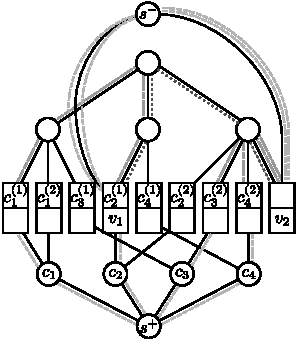
\includegraphics[width=\columnwidth]{figs/flow_ma_cv}
\caption{Example of flow construction: Problem instance with two nodes, four chunk
types, and two replicas per type. The min-cost-max-flow
is indicated by the dotted lines: each line represents one unit of flow.
\maciek{Float this figure, perhaps even scale down.}
}
\label{fig:flow_construction}
\end{figure}

\textbf{Algorithm.}
Our algorithm to solve $\RS+\MA+\CC+\BW$ consists of three parts:
\emph{First}, we construct the normalized and extended graph $\Tree^*$
described above and compute
a min-cost-max-flow solution, e.g., using~\cite{mincostmaxflow-1,mincostmaxflow-2}.
\emph{Second}, we have to \emph{round} the resulting, possibly fractional flow, to
integer values. Due to the \emph{integrality theorem}~\cite{flow-book},
there always exists an optimal integer solution on graphs with integer capacities.
However, while algorithm like the successive shortest path algorithm~\cite{successive_shortest_path_complexity}
directly give us such an integral solution (in polynomial time), the fastest min-cost-max-flow algorithms (e.g., based on double-scaling
methods~\cite{mincostmaxflow-1} or minimum mean-cost cycle algorithms~\cite{mincostmaxflow-2} \maciek{mean-cost cycle algorithm is AFAIK designed to solve specific flow problem where we have negative costs; we only have costs 0 or 1, so this algorithm might not  be the best example}), may yield fractional solutions
which need to be rounded to integral solutions (of the same cost).
In order to compute integral solutions, we proceed as follows: we iteratively pick an arbitrary (loop-free \maciek{We will not have any loop in our flow because all edge costs are non-negative}) path
currently having a fractional allocation of value $f$ ($f>0$), and distribute its flow $f$
among all other fractional paths of the same length; due to the optimality of the fractional solution
and due to the integrality theorem, such paths must always exist. After distributing this flow,
the total allocation on this path will be 0, and we have increased the number of integer paths by one.
(In addition, some paths may now have an integer allocation of 1.) We proceed inductively.
\emph{Third}, given an integer min-cost-max-flow solution, we need to decompose the integer flows into the paths
representing matched chunk-node pairs:
The assignment can be obtained by decomposing the flow allocated in the
original substrate network\maciek{Passive voice - consider rewrite.}
. In order to identify a matched chunk-node pair,
we take an arbitrary (loop-free) path $p$ carrying a flow of value  $\geq 1$ from $\Source$ to $\Sink$:
the first hop represents the chosen chunk type, the second hop the chosen
replica, and the last but one hop represents the server: we will assign
the replica to an arbitrary unused node on this server.
Having found this pair, we reduce the flow
along the path $p$ by one unit.
We continue building the pairing by selecting replicas until every chunk type is processed.

\textbf{Analysis.}
The correctness of our approach follows from our construction
of $\Tree^*$, using integer capacities (in our case $\lfloor\capacity(e)/\CostTrans\rfloor$),
and the fact that cost optimal integral solutions always exist~\cite{flow-book}.
The runtime of our algorithm consists of four parts: construction of $\Tree^*$,
computation of the min-cost-max-flow, flow rounding, and decomposition. The
dominant terms in the asymptotic runtime is the flow computation.
Using the state-of-the-art min-cost-max-flow algorithms~\cite{mincostmaxflow-1,mincostmaxflow-2}
we get a runtime of $\mathrm{O}(n_S^2 \cdot \log\log \min \{U,\tau\})$ 
 \maciek{Double check that!}
where $U$ is the maximal link capacity; note that in networks with high capacity and uncapacitated networks, we can simply
 set $U=\tau$.
% resp.~$\mathrm{O}(n_S^5 \cdot \tau^3 \log n_S)$, where $\delta$ is the network diameter and
%where $U$ is the maximal link capacity in the substrate;
%using~\cite{successive_shortest_path_complexity},
%together with the Dijkstra shortest-path algorithm we have $\mathrm{O}(n_S^2\cdot \tau)$.

%\textbf{Summary.}
%Figure~\ref{fig:venn_flow} summarizes all problem
%variants which can be solved with our flow-based approach.

\subsection{Matching Algorithms ($\RS+\MA+\CC$ and $\MA+\CC+\BW$)}\label{ssec:match}

\begin{wrapfigure}{r}{0.5\columnwidth}
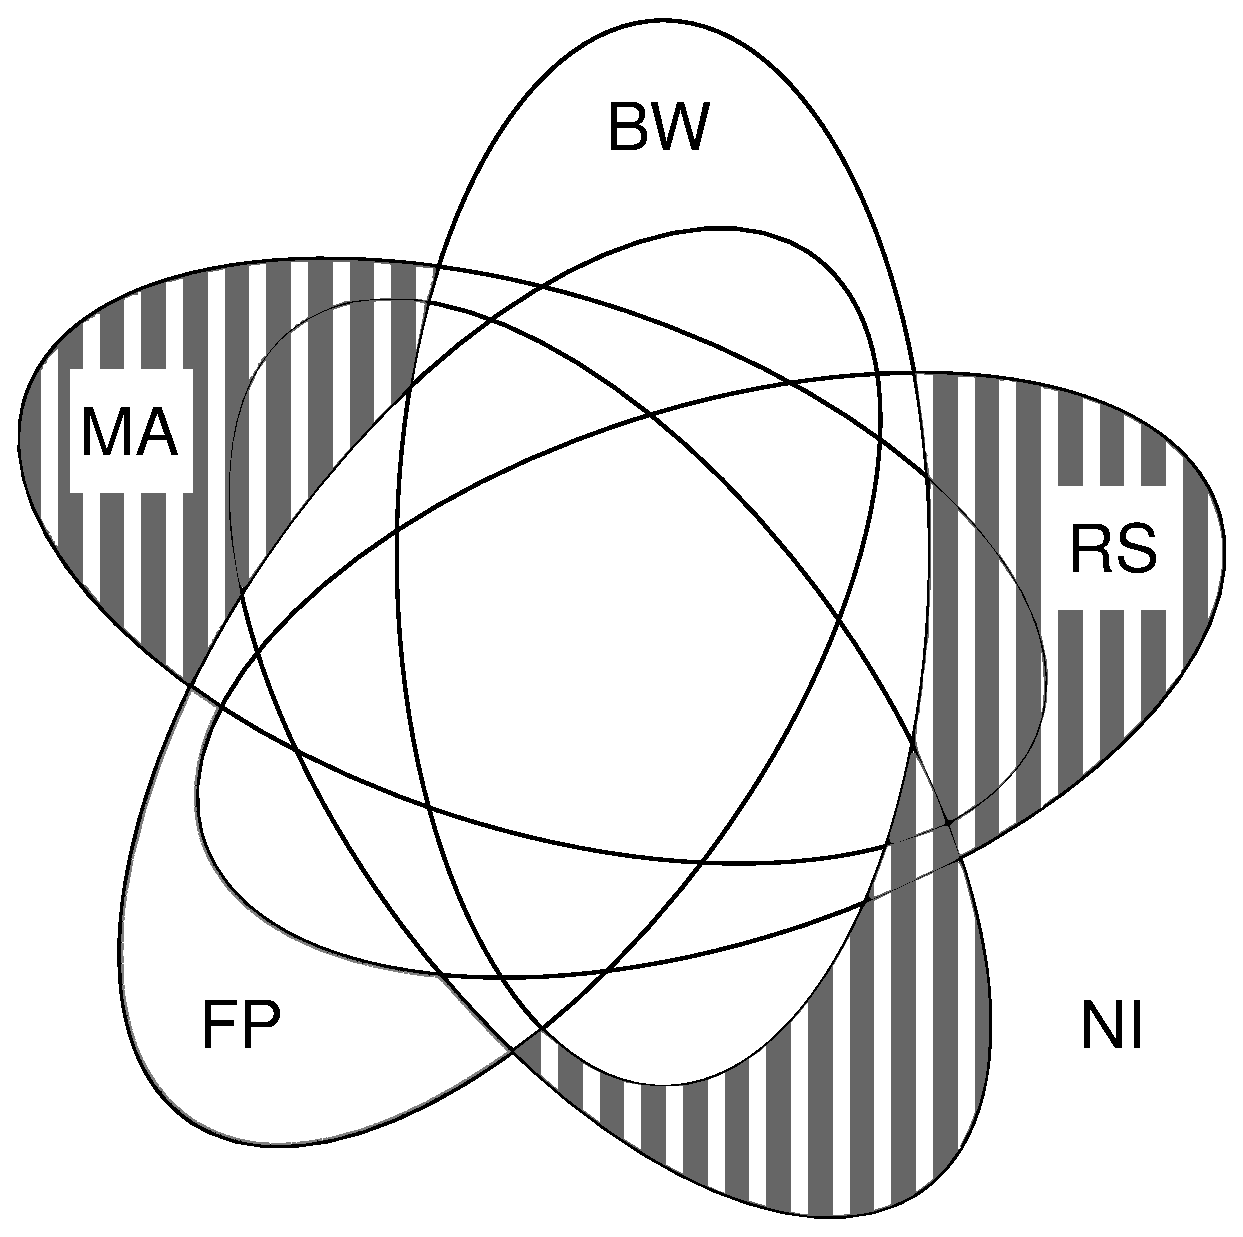
\includegraphics[width=0.48\columnwidth]{figs/venn_matching.pdf}
\caption{Variants solved by matching approach.\maciek{There is no $\MA+\CC+\BW$ marked in this diagram.}}
\label{fig:venn_match}
\end{wrapfigure}

This section presents faster algorithms to solve the two problem variants
$\RS+\MA+\CC$ and $\MA+\CC+\BW$ which can also be solved with the flow approach
introduced above.
In general, the algorithms presented in this section can be summarized
as matching approaches\maciek{Passive voice - consider rewrite.}
.

\subsubsection{$\RS+\MA+\CC$}

Let us first consider the $\RS+\MA+\CC$ variant.
Recall that in this problem,
we are given a set of redundant chunks ($\RS$) and a set of nodes
at fixed locations. The number of chunk types is larger than the number
of nodes ($\MA$), and each node needs to be connected
to its chunks as well as to other nodes ($\CC$).
Our goal is to minimize the resource footprint $\Cost$, consisting
of the bandwidth reservations in the access network and the inter-connect.

\textbf{Algorithm.} Due to Observation~\ref{obs:nofp}, $\RS+\MA+\CC$ degenerates to $\RS+\MA$.
In order to solve the $\RS+\MA$ problem variant,
we construct a bipartite
graph between the set
$\VirtualNodes$ of nodes and
the set of chunks.
Concretely, we clone each node $\MaFactor$ times,
as each node needs to process
$\MaFactor$ chunk types, and we collect all copies of a given chunk type in a
single %$\ChunkType$
``super-node''. We connect each node to all chunk types using the
\emph{lowest hop count} to one of the copies as the cost metric (the link weight).

On the resulting graph, we can now compute a \emph{Minimum Weight
Perfect Bipartite
Matching}~\cite{gabow_scaling_algorithm}:
the resulting matching describes the optimal assignment of chunks to nodes. \maciek{Minimum Weight Perfect Matching in bipartite graph}

%\begin{figure}[h]
%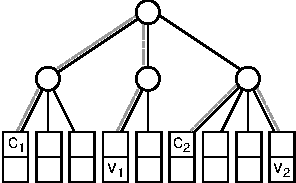
\includegraphics[width = 0.49\columnwidth]{figs/matching_topology_simple}
%\hfill
%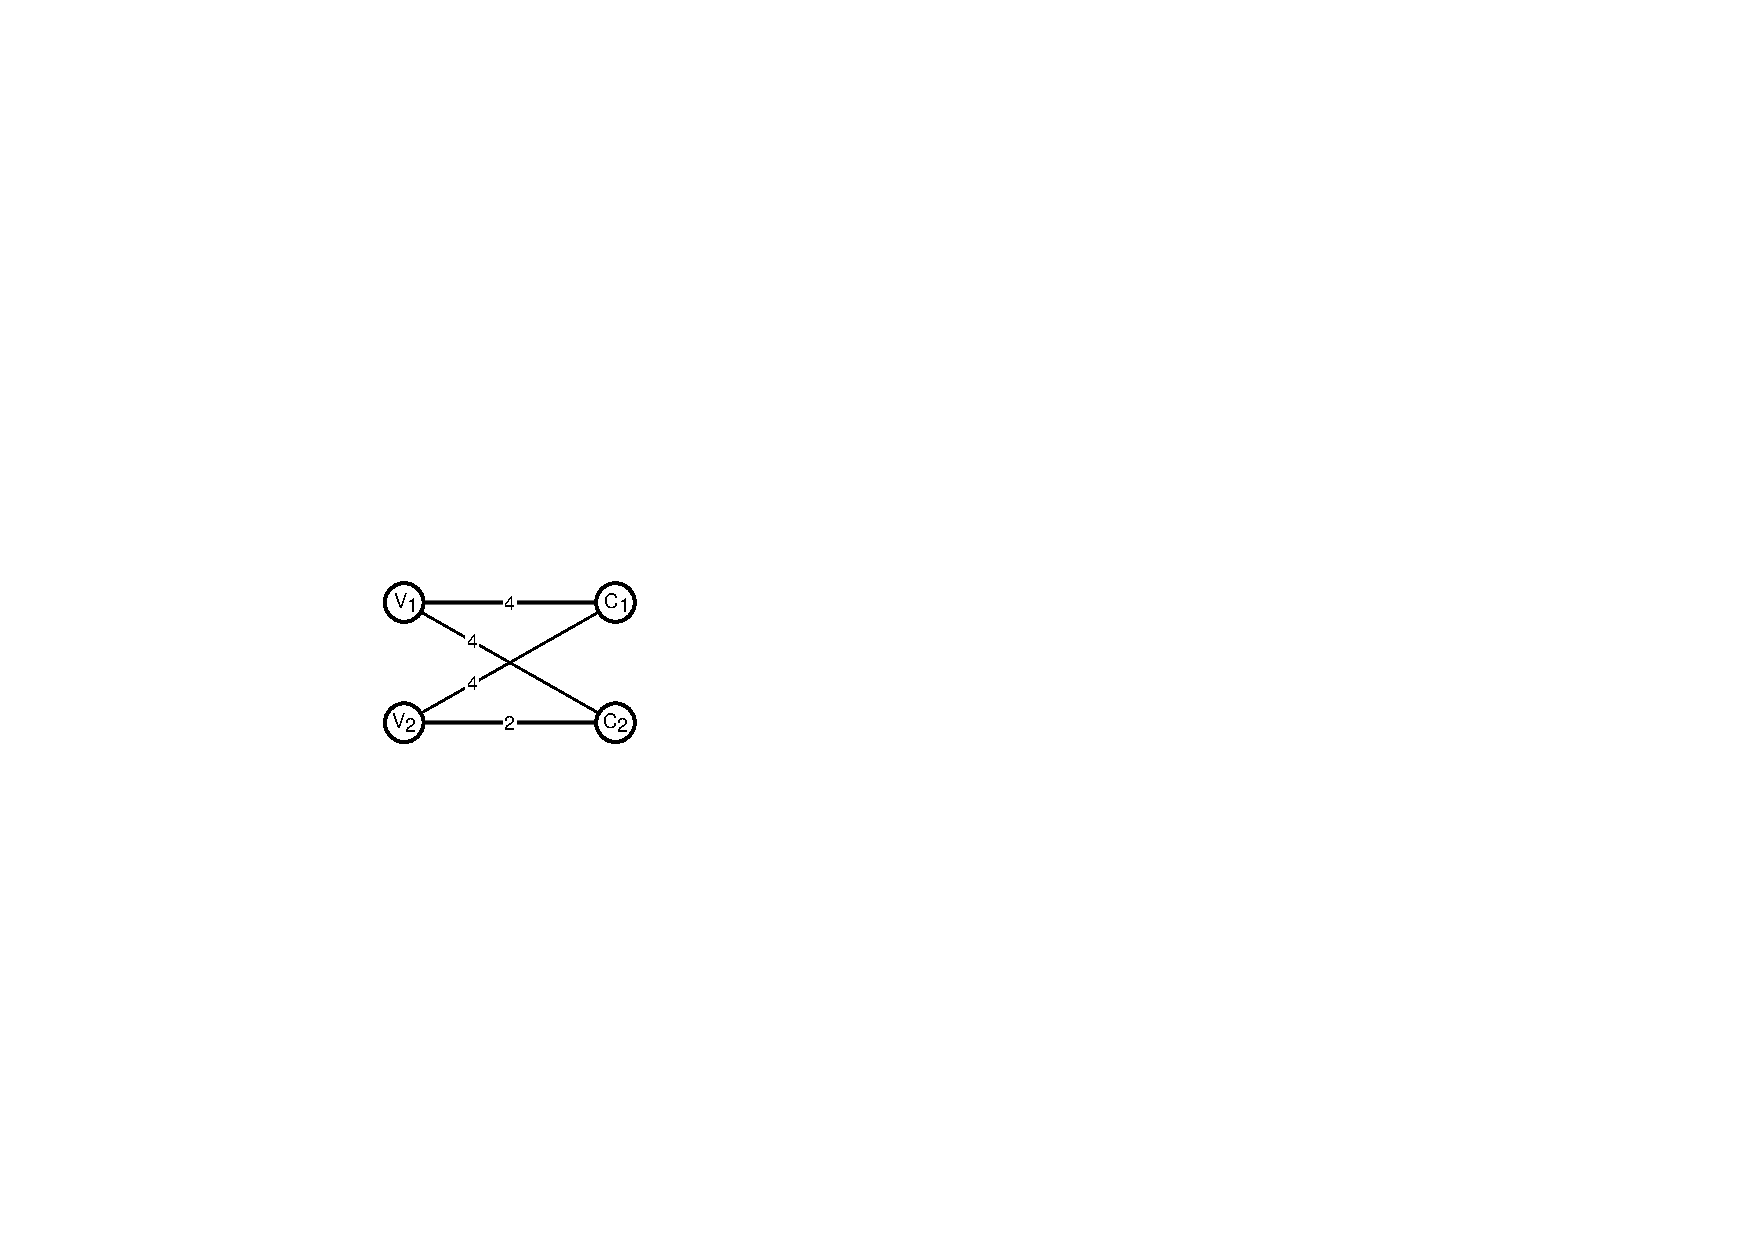
\includegraphics[width =0.4\columnwidth]{figs/matching_basic}
%\caption{The problem instance on the \emph{left} consists of
%two nodes and two chunks. The
%optimal solution is indicated by the dashed lines. The corresponding matching
%problem on the \emph{right} represents the same situation. The weights on the
%edges
%are set according to the distance in the substrate. The solution of the minimum
%cost perfect matching is depicted by the shaded lines.}
%\label{fig:matching_basic}
%\end{figure}

\begin{figure}
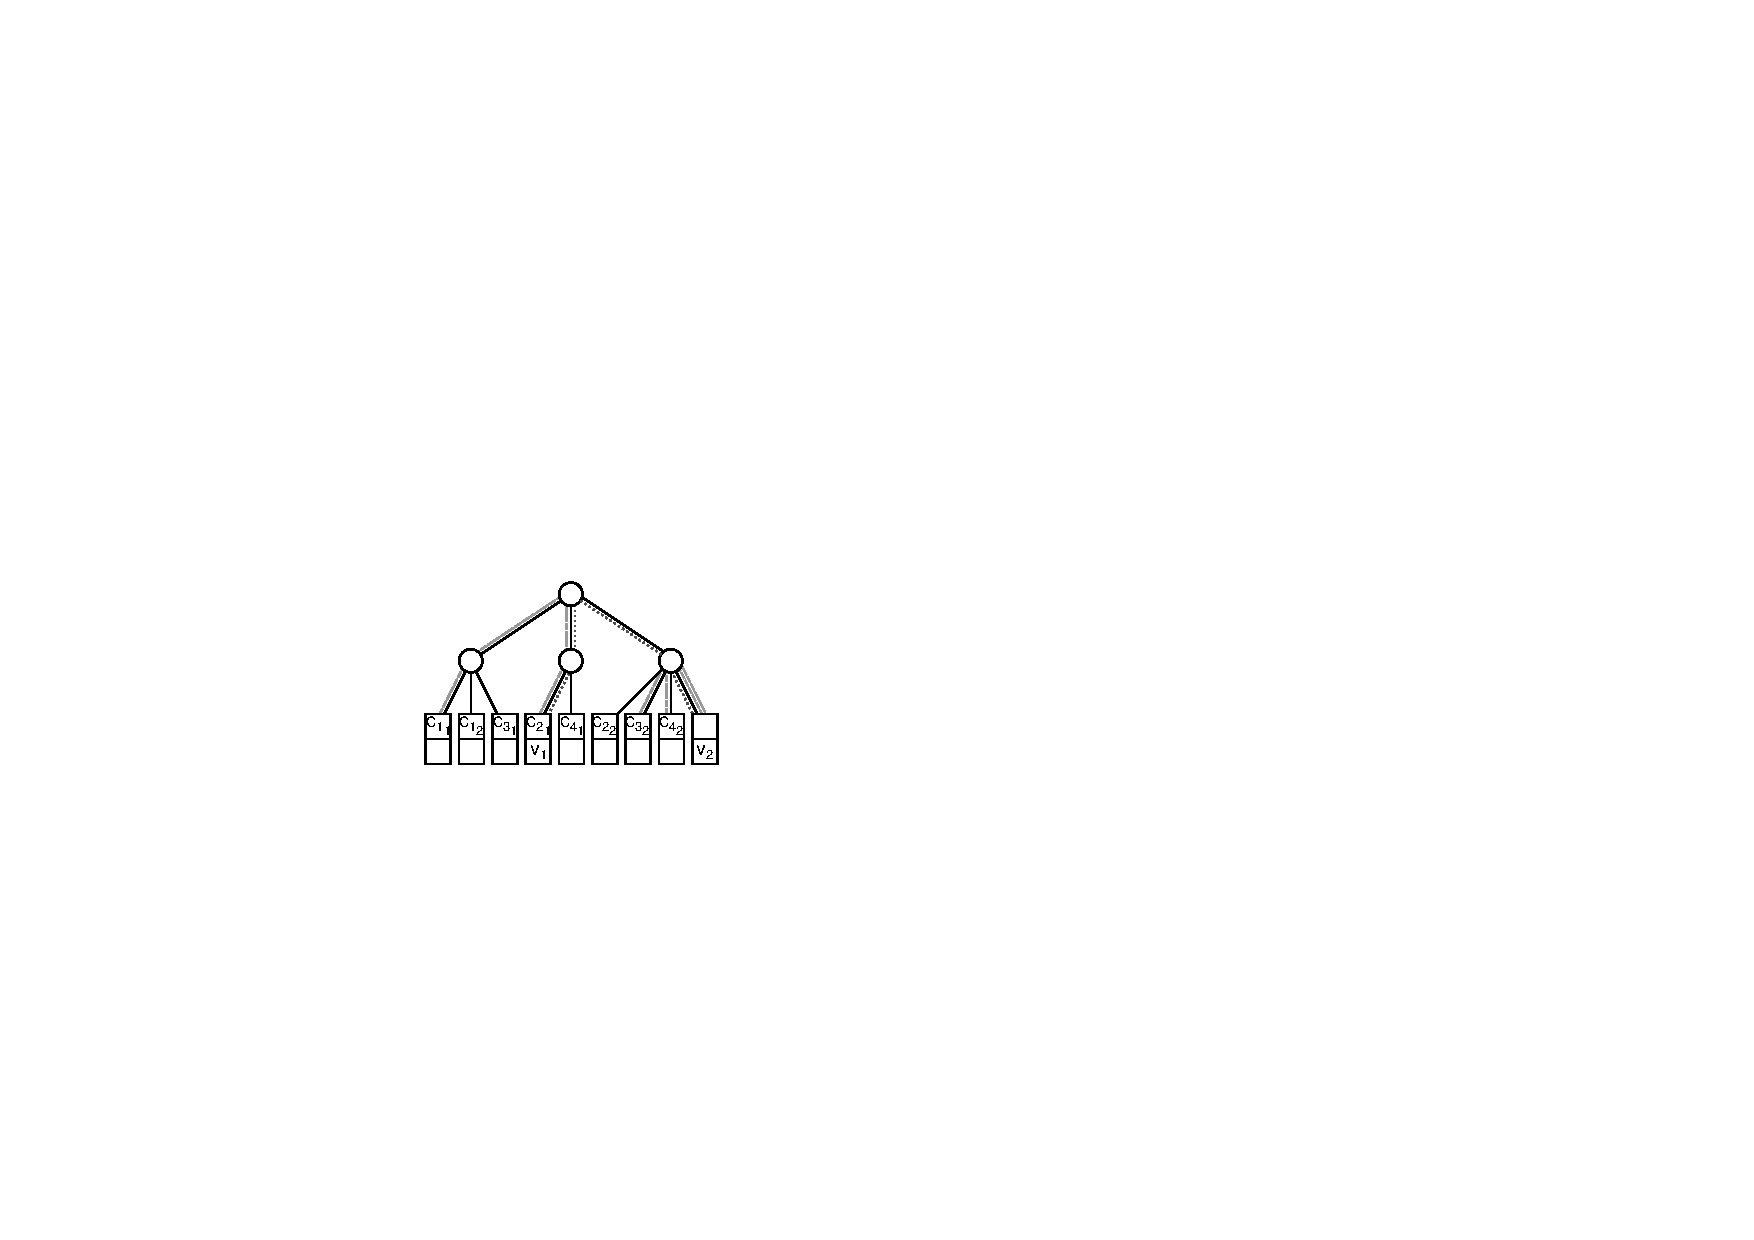
\includegraphics[width = 0.49\columnwidth]{figs/model_ma_r_cv_boxes}
\hfill
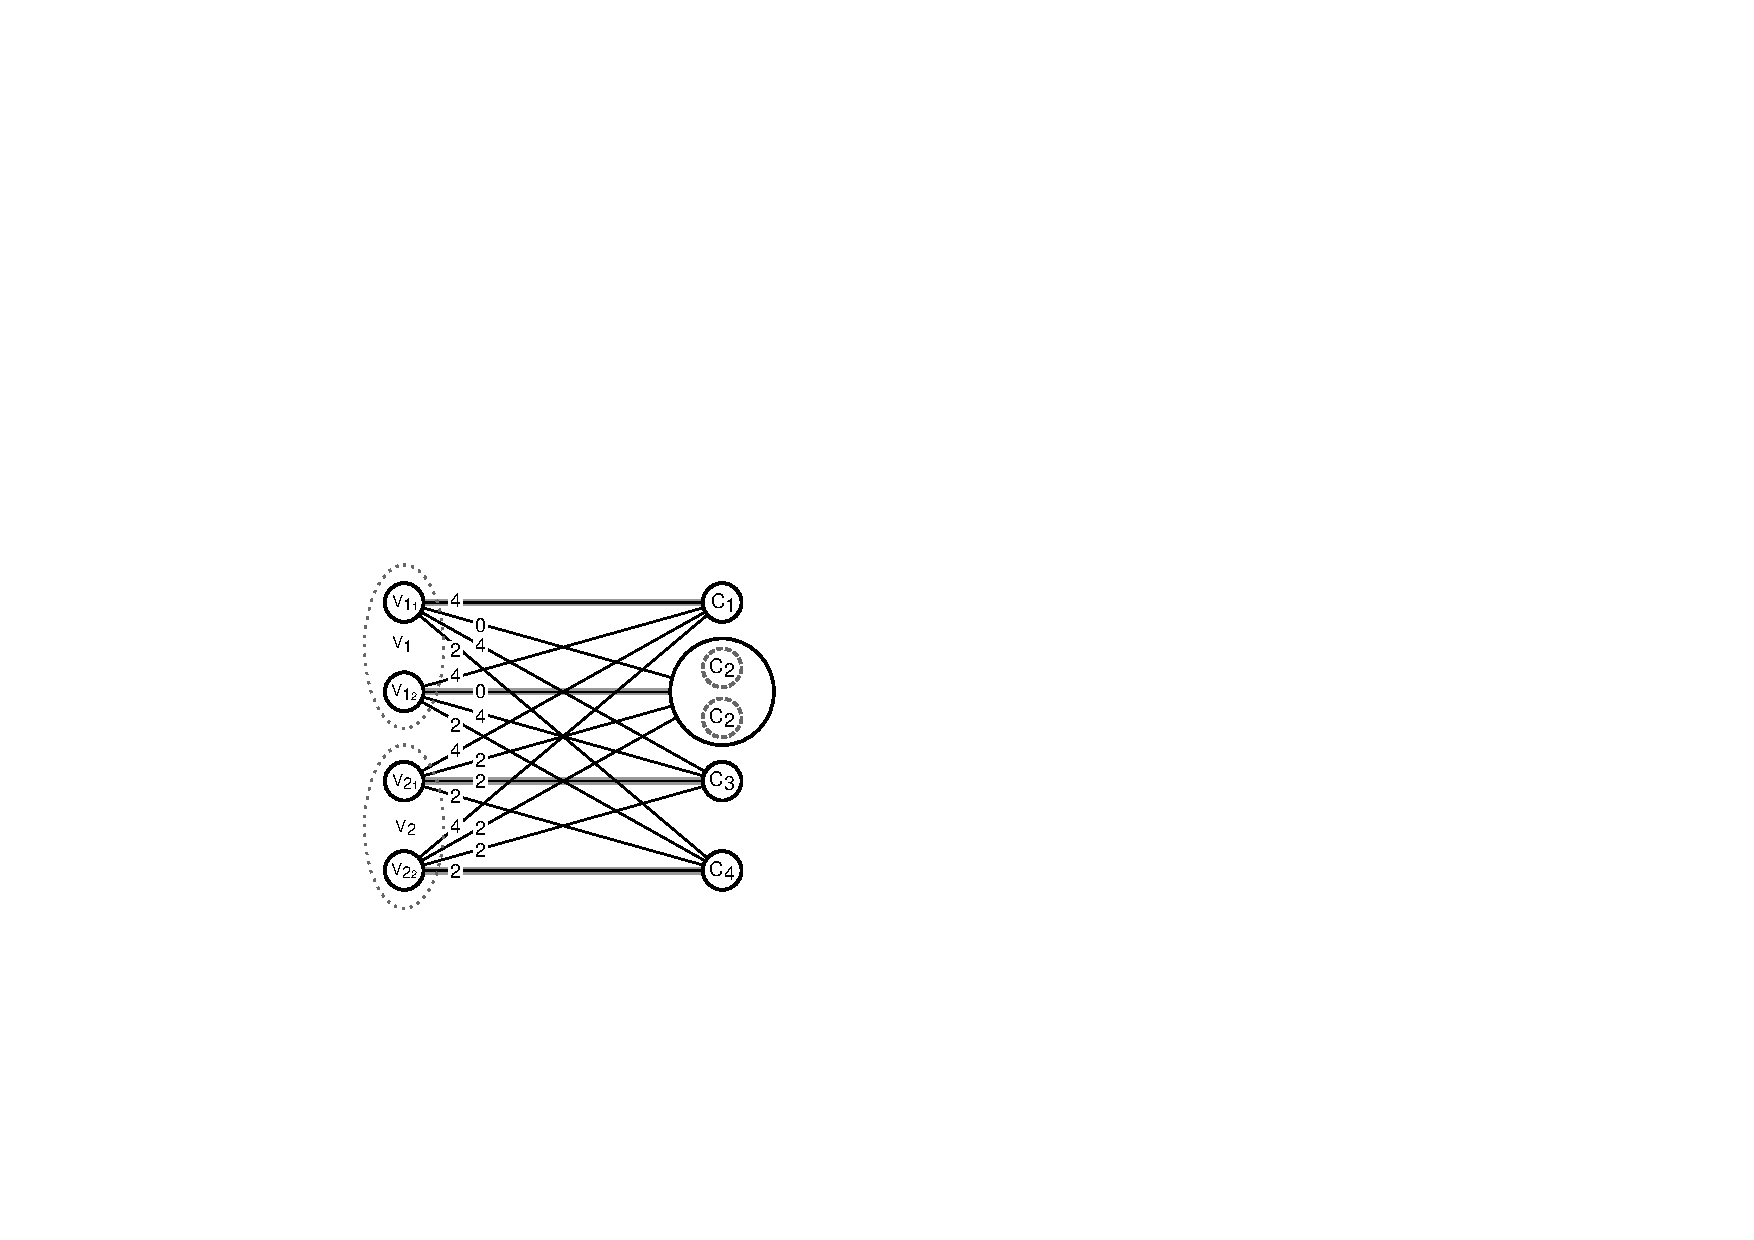
\includegraphics[width =0.49\columnwidth]{figs/matching}
\caption{The $\MA+\RS$ problem on the \emph{left} is converted into a
matching problem on the \emph{right}. Since each node has to process two
chunks, the
nodes are replicated in the matching representation. The two replicas of each
chunk type are represented by a single node, and all edges connecting to this
node have a weight according to the shorter distance to one of the replicas.
This is visualized for $\achunk_2$.\maciek{Consider scaling up the figure. Or even putting the tree above the graph.}}
\label{fig:matching}
\end{figure}

\textbf{Example.} Before analyzing our algorithm, let us consider a small example.
%
%Figure~\ref{fig:matching_basic} shows an example:
%$\NodeMapping(\VirtualNode_1)$ is four hops
%away from all chunks; in the matching problem, this is
%reflected in the corresponding edge
%weights. Similarly, $\NodeMapping(\VirtualNode_2)$ is
%two hops away from $\achunk_2$, and four hops away from $\achunk_1$. Hence the
%weight of the edge $(\NodeMapping(\VirtualNode_2),\achunk_2)$ is $2$, while the
%weight on the edge to $\achunk_1$ is $4$. The solution to the minimum weight
%perfect bipartite matching contains the edges $(\NodeMapping(\VirtualNode_1),
%\achunk_1)$ and $(\NodeMapping(\VirtualNode_2),
%\achunk_2)$, which is exactly the optimal chunk to node assignment
%$\VmChunkAssignment$,
%visualized using dashed lines in Figure~\ref{fig:matching_basic}.
%
%\begin{figure}
%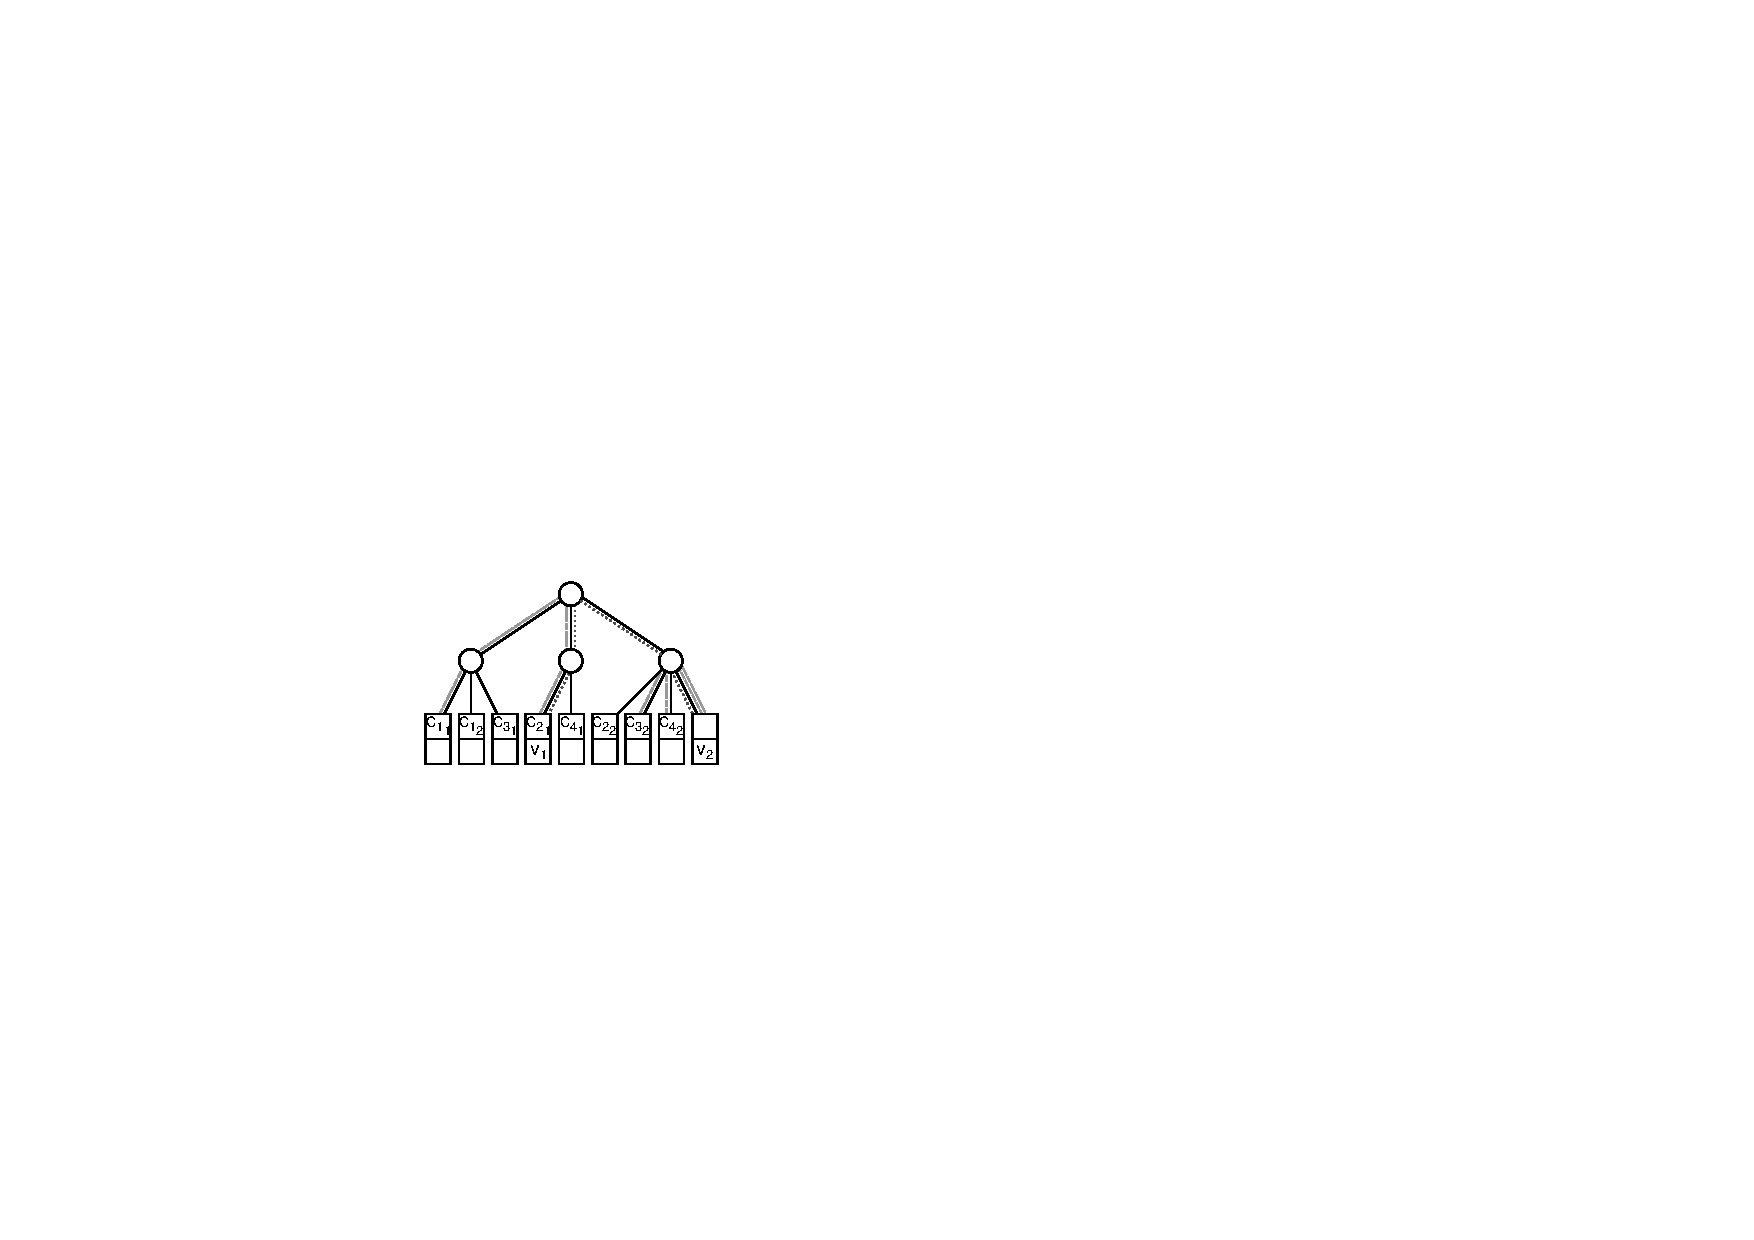
\includegraphics[width = 0.49\columnwidth]{figs/model_ma_r_cv_boxes}
%\hfill
%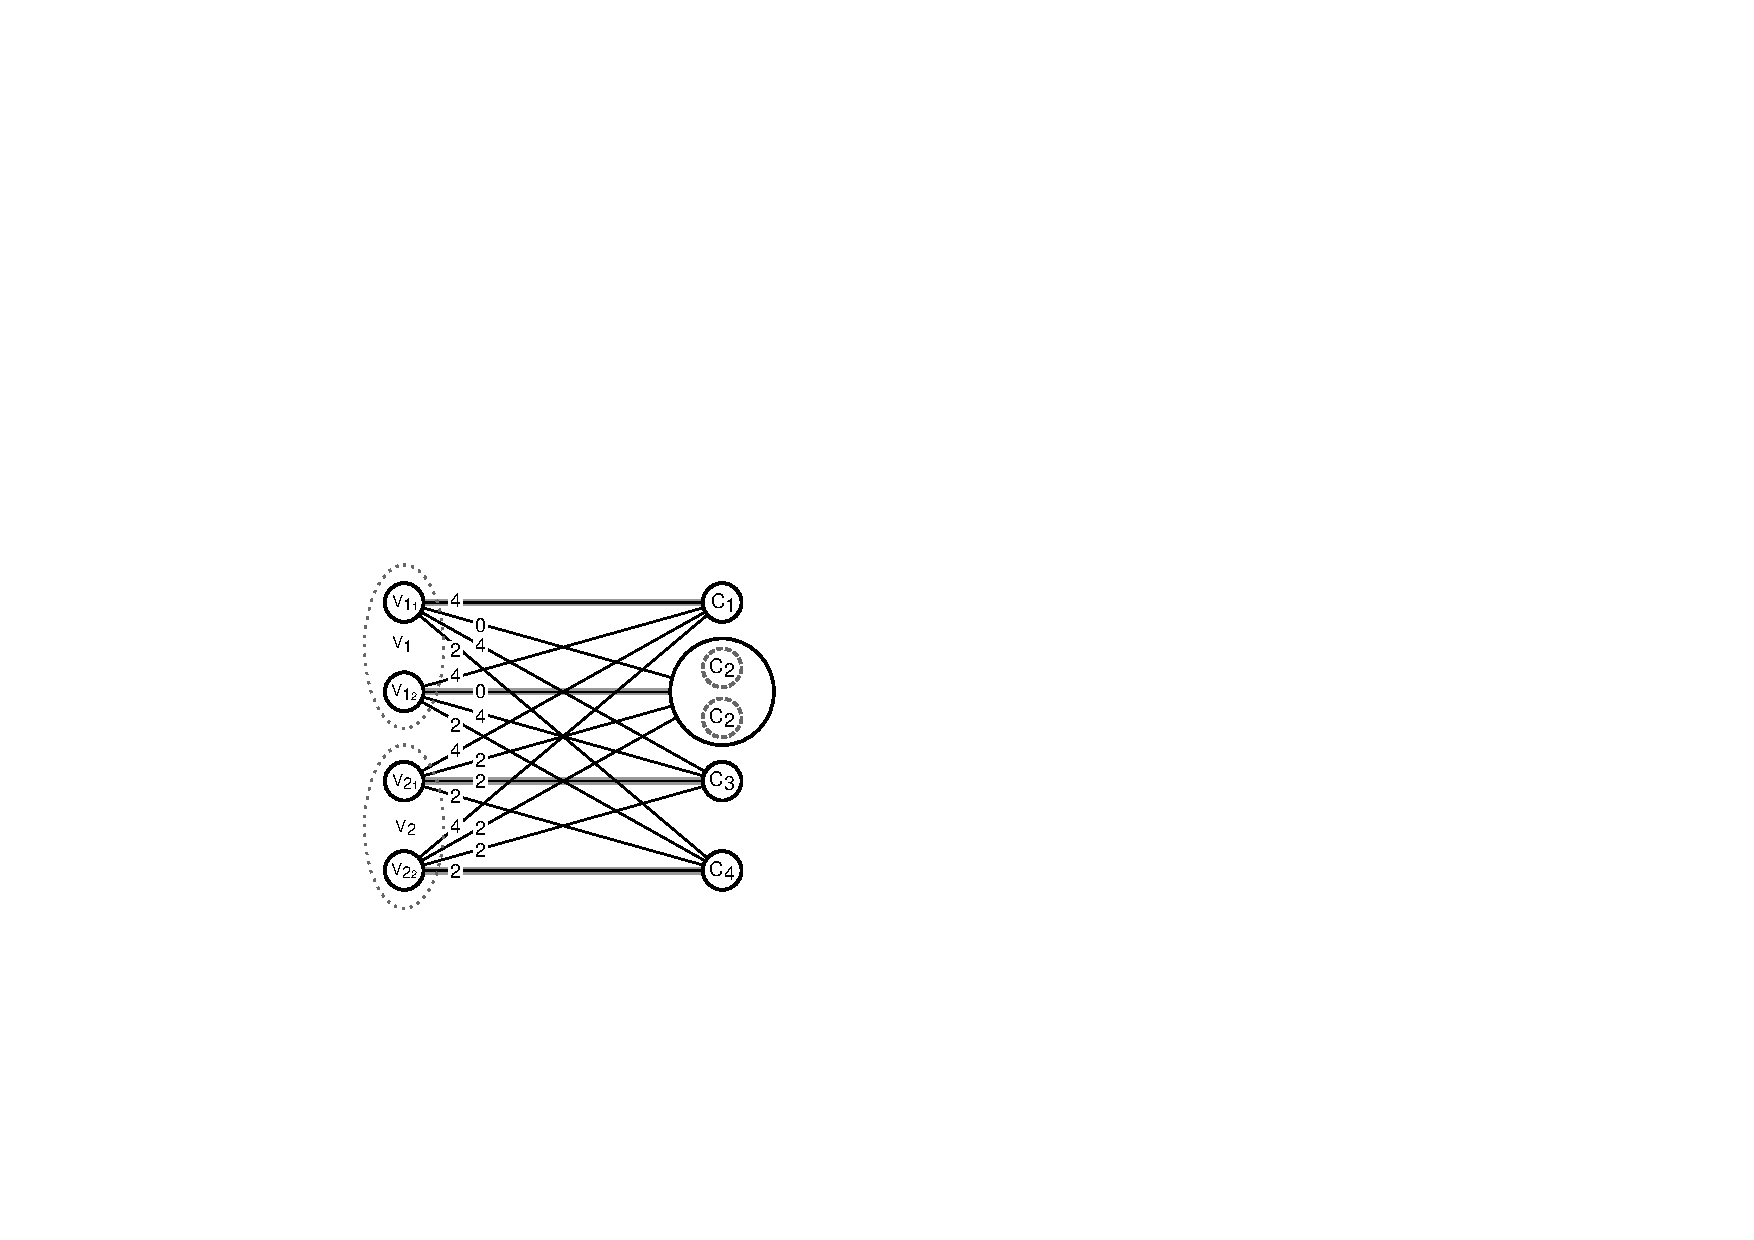
\includegraphics[width =0.49\columnwidth]{figs/matching}
%\caption{The $\MA+\RS$ problem on the \emph{left} is converted into a
%matching problem on the \emph{right}. Since each node has to process two chunks, the
%nodes are replicated in the matching representation. The two replicas of each
%chunk type are represented by a single node, and all edges connecting to this
%node have a weight according to the shorter distance to one of the replicas.
%This is visualized for $\achunk_2$.}
%\label{fig:matching}
%\end{figure}
%
Figure~\ref{fig:matching} illustrates
%the procedure for a more complex problem
an instance where two nodes are
cloned into $\MaFactor = 2$ nodes each, resulting in a total of four nodes in
the matching problem representation.
The $\RedundancyFactor = 2$ chunks of each chunk type are
aggregated into a single chunk type node $\achunk_j$  in the matching problem;
this gives a total of four chunk type nodes in the matching graph. The costs
on the links between all clones of a specific node and a chunk type are set to
the minimum distance. This can for instance be observed\maciek{Remove passive voice - We can observe that for instance} at the edges connecting
the two clones of $\VirtualNode_1$ to $\achunk_2$: both weights are 0.

\textbf{Analysis.}
%Let us now study the runtime of the matching approach.
The correctness of our algorithm follows from the construction and the optimal
solution of the minimum matching.
The runtime consists of two parts: the construction of the matching graph and
the actual matching computation. The constructed graph consists of
$\MaFactor \cdot n_V \cdot \ChunkType$ many edges,
and for each edge we need to compute its cost, i.e., the shortest distance
which in a tree can be computed in time $n_S$\maciek{Passive voice - consider rewrite.}
; thus, the overall construction time
is
%$\mathrm{O}(n_S \cdot \MaFactor \cdot n_V \cdot \ChunkType)$.
$\mathrm{O}(n_S \cdot \tau^2)$.
The state of the art algorithm to compute matchings are based on scaling techniques.~\cite{scale-match}
The runtime translates to
%graph $n$, the number of edges in the graph $m$, and the largest magnitude of
%an edge weight $N$. An efficient algorithm is described by Gabow et al. in
%\cite{gabow_scaling_algorithm} and provides a runtime of
%$\mathcal{O}(n_S^{3/4} \cdot \lambda \cdot \log \delta)$, where $\delta$ is the network diameter
%and where $\lambda= \MaFactor \cdot n_V \cdot \ChunkType$ represents the number of edges in the matching graph.
%$\mathcal{O}(\tau^{11/4}*n_S)$,
$\mathcal{O}(\tau^{5/2}\cdot \log(\tau\cdot n_S))$.
%where $C$ is the maximal link capacity.
(Recall that $\tau = \MaFactor\cdot n_V$.) \maciek{Double check that.}


%\begin{comment}
%The following lemma essentially states that any non-local matching can only have higher
%costs in all subtrees.
%
%\maciek{We need to introduce what we mean by partial matching before
%  formulating this lemma.}
%\begin{lemma}\label{lemma:local}
%A local and greedy perfect matching of chunks to nodes is optimal.
%\end{lemma}
%\begin{proof}
%Proof by contradiction. Let us assume that there exists an optimal matching $M'$ of cost lower
%than the local greedy matching $M$.
%Let us consider the smallest subtree where the (partial) matching of $M$
%has a different cost than the (partial) matching of $M'$.
%This means
%that a non-local decision was made by $M'$ in this subtree (hoping for savings higher up),
%and there must exist two matched pairs in $M'$ that shares a link (one pair is transporting a chunk up, and
% the other one a chunk down). Then we can create a matching $M''$
% which uncrosses these edges of $M'$ (i.e., does the local matching on them),
%  and is cheaper than $M'$. Contradiction.
%\end{proof}
%
%\end{comment}

\subsubsection{Faster $\MA+\CC$ and $\MA+\CC+\BW$}

We now show that we can solve $\MA+\CC$ even faster, by exploiting
locality. Moreover, we will show that
even
$\MA+\CC+\BW$ problem variants can be solved with our approach, by simply
verifying feasibility\maciek{Passive voice - consider rewrite.}
.
In the following, due to Observation~\ref{obs:nofp}, we can focus on
the $\MA$ resp.~$\MA+\BW$ problem.

We first need the following definition \maciek{Rewrite this sentence.}.
\begin{defn}[Local Assignment (LA)]\label{def:loc}
We define an assignment $\VmChunkAssignment$ to
be \emph{local in a specific subtree $\Tree'$}, iff~$\VmChunkAssignment$
assigns the maximum number of chunks in the
subtree to nodes in the same subtree.
% (subject only to the number of available nodes
%in $\Tree'$).
We define $\VmChunkAssignment$ to be \emph{local} when
it is local with respect to all possible subtrees of the substrate network.
\end{defn}

\begin{figure}
\center
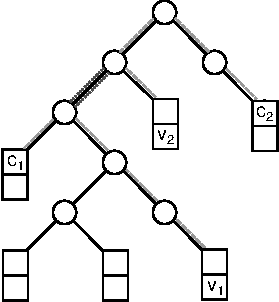
\includegraphics[width = 0.6\columnwidth]{figs/unbalanced_tree}
\caption{Illustration of local assignment: The dashed lines indicate bandwidth allocations, which occur
independently of the chosen assignment. The dotted lines indicate bandwidth
allocation which occur only if $c_2$ is assigned to $v_1$.}
\label{fig:unbalanced_tree}
\end{figure}

\textbf{Example.}
Figure \ref{fig:unbalanced_tree} illustrates the concept of local assignment:
The closest chunk to $v_2$ is $c_1$, and the closest node to $c_1$ is $v_2$. 
However, a subtree $T'$ exists such that $v_1 \in T'$ and $c_1
\in T'$, but $v_2 \notin T'$. Therefore, a local assignment cannot assign $c_1$ to $v_2$.

% shows an instance with two chunks and
%two nodes. A local assignment assigns $v_1$ to $c_1$, although $c_2$ is
%closer to $v_1$, since a subtree $T'$ exists, 


We will see later that
optimal solutions to
$\MA$ have a local assignment. This is exploited by our algorithms described
in the following.

\textbf{Algorithm.} Our proposed algorithm for $\MA$
proceeds in a bottom-up fashion, traversing the substrate network $\Tree$
from the leaves toward the root.
For each subtree $\Tree'$, we maintain
two sets $S_1,S_2$ in order to match unmatched
chunks $S_1$ in the subtree $\Tree'$ to unmatched
nodes $S_2$ in $\Tree'$. Both sets are initially empty.

We first process all the leaves, in an arbitrary order; subsequently, we process arbitrary inner vertices
of $\Tree$, whenever all their children have been processed.
We process any leaf $\ell$
by adding any
nodes or chunks which are located on $\ell$ to the corresponding sets $S_1$ and $S_2$.
A non-leaf vertex $u$ is processed in the following way: we take the union of
the sets of $u$'s children, i.e., the sets contain the unmatched chunks and nodes
in this subtree.
For both leaves and inner nodes, whenever
both sets are non-empty, we greedily match an arbitrary chunk in $S_1$ with an arbitrary node in $S_2$,
and remove them from the sets.

\textbf{Analysis.} On a given vertex $u$, emptying one of the sets, results in a \emph{local assignment} (cf~Definition~\ref{def:loc})
in the
subtree rooted at $u$. Due to our bottom-up strategy, the overall assignment
will also be local.
The complexity of this
construction is low: For each
vertex in the substrate graph,
we have to\maciek{We build the union (no ``have to'')} build the union of the children's sets,
and since each vertex can only be the child of one vertex,
the amortized runtime per vertex is constant; and hence the overall
runtime $\mathcal{O}(n_S)$. The sum of all remove operations, is equal to
the number of chunk types $\mathcal{O}(\ChunkType)$.
Hence the overall complexity of this construction amounts to
$\mathcal{O}(n_S + \ChunkType)$.

It remains to prove optimality of such local assignments.
We first characterize the bandwidth allocation on uplinks of subtrees.
\begin{lemma}\label{lem:uplink-alloc}
Given an $\MA$ problem and a subtree $\Tree'$
containing $x$
chunks and $y$ nodes, the minimal bandwidth allocation of any
assignment
$\VmChunkAssignment$ on the uplink of $\Tree'$ is $|x-y\cdot\MaFactor|\cdot
\CostTrans$. \label{lemma:uplink}
\end{lemma}
\begin{proof}
  If number of chunk types equals the processing capacities of the nodes in the given subtree,
the bandwidth allocation inflicted by the chunk access network on the uplink can be
zero, since all chunks can be assigned to nodes in the same subtree\maciek{Passive voice - consider rewrite.}
.
Otherwise, we distinguish between two cases: Recall, that in instances
without $\RS$, all chunks have to be processed. In case
there are more chunks in the subtree, at least all of the excess chunks have to
be transferred to a different subtree, which will
inflict costs $\CostTrans$ per excess chunk on the uplink connecting $\Tree'$
with the
remaining parts of $\Tree$. Similarly, if the processing capabilities exceed the
amount of
available chunks, excess chunks from other subtrees will have to be transferred
to
nodes in the subtree $\Tree'$, inflicting bandwidth costs of $\CostTrans$ each.
Hence, the minimum bandwidth allocation for the chunk transport on the uplink
is the difference between the number of chunks and the processing capabilities
of the subtree $|x-(y\cdot\MaFactor)|$ \maciek{we can drop the parenthesis like in formulation of the lemma} times the amount of bandwidth needed,
for a single transfer $\CostTrans$.
\end{proof}


\begin{theorem}
Given an $\CC+\MA$ problem instance, a feasible assignment $\VmChunkAssignment$
is optimal iff it is local.
\label{thm:local_optimal}
\end{theorem}

\begin{proof}
Local assignments generate exactly the minimal allocations on all links, as described in
the proof of
Lemma~\ref{lemma:uplink}. Hence
each local assignment has to be optimal. A non-local assignment, has at least
one subtree, in which it is not local. This subtree will have a higher
allocation on the uplink. Since the local assignment has minimal allocations
on all other links, the non local assignment has a larger footprint.
\end{proof}


%\begin{comment}
%Since each link is an uplink of one subtree,
%Lemma~\ref{lem:uplink-alloc} implies:
%\begin{corollary}
%All local assignments result in the same cost, for any $\CC+\MA$ problem instance.
%\label{corollary:same_costs}
%\end{corollary}
%
%
%
%
%\stefan{TODO: Describe unbalanced tree pic}
%
%We can now prove optimality:
%\begin{theorem}
%Given an $\CC+\MA$ problem instance, a feasible assignment $\VmChunkAssignment$
%is optimal iff it is local.
%\label{thm:local_optimal}
%\end{theorem}
%\begin{proof}
%By contradiction. We will show, that a non-local assignment is not optimal. Combined with
%Corollary~\ref{corollary:same_costs}, this results in the optimality of all
%local assignments.
%
%Assume a non-local optimal assignment $\VmChunkAssignment$ exists.
%This means, for at least one subtree, it assigns
%a chunk $\achunk_i$, located in the subtree, to a node $\VirtualNode_i$ outside
%the
%subtree. In addition,
%at least one node $\VirtualNode_j$ in the subtree has to process a chunk
%$\achunk_k$ located outside the subtree. We construct an alternative
%assignment $\VmChunkAssignment'$, by exchanging the assignments of
%$\achunk_i$ and $\achunk_j$. Since $\achunk_i$ is located in a subtree which
%contains $\VirtualNode_j$ but not $\VirtualNode_i$, and both nodes and chunks
%are only located at leaves, the distance between $\achunk_i$ and its assigned
%node is smaller in $\VmChunkAssignment'$. For the distance between $\achunk_j$
%we make a case distinction: if there exists a subtree which
%contains $\achunk_i$, $\achunk_j$ but not $\VirtualNode_i$, the distance
%between $\achunk_i$ and $\VirtualNode_i$ is equal to the distance between
%$\achunk_j$ and $\VirtualNode_i$. Since $\achunk_i$ is closer to
%$\VirtualNode_j$ than $\achunk_j$, the overall costs of $\VmChunkAssignment'$
%would be lower in this case. If the described subtree does not exist, the
%distance between $\achunk_j$ and the two nodes is the same, which
%renders $\VmChunkAssignment'$ cheaper than an optimal
%solution. Contradiction.
%\end{proof}
%\end{comment}

Combined with a simple postprocessing step, this approach can also solve $\MA+\BW$. The central idea of this extension, is
that \emph{local} assignments allocate the minimal bandwidth
on each individual edge. In consequence, each bandwidth constraint
which is lower than the allocation of a local assignment on one link, renders
the problem infeasible. Hence, it is sufficient to temporarily omit the
bandwidth limitations, compute an optimal assignment for an $\MA$ instance, and
verify that the resulting allocations do not violate any capacities. The
postprocessing step scales linearly with the number of edges in the substrate
graph.\maciek{The postprocessing time scales linearly with respect to the number of edges in the substrate graph.}
%Due to the tree topology of the substrate graph, the number of
%edges in the substrate is $n_S - 1$, which does not affect the
%asymptotic complexity of this approach.}

%\begin{comment}
%to show
%that if the \emph{local} assignments violates the available bandwidth on any
%link, all other assignments will also violate the bandwidth. As a consequence
%it is possible to simply compute the assignment without any bandwidth constraints, and
%check in a postprocessing step, whether the bandwidth on any link is exceeded.
%This postprocessing step scales with the number of edges in the substrate,
%which is lower than the number of nodes in the substrate.
%Hence the asymptotic runtime of the approach does not change.
%
%
%\stefan{fix the following! also note that the notation $F(...)$ has not been introduced!}
%
%\begin{lemma}
%Given a minimal cost assignment $\VmChunkAssignment$,
%any solution with bandwidth allocation less
%than $\Cost(\VmChunkAssignment,
%\SubstrateEdge)$ to any link renders the problem
%infeasible.
%\label{lemma:no_bandwidth}
%\end{lemma}
%\begin{proof}
%From Lemma~\ref{lemma:uplink} we know that each optimal assignment
%$\VmChunkAssignment$ to $\MA+\CC$ assigns a certain bandwidth to a link. This is
%the minimal bandwidth which has to be allocated on this link by \emph{any}
%feasible assignment, since removing the locality, can only increase the number
%of chunks which have to be transported across the uplink.
%Assume there exists a link on which the assignment $\VmChunkAssignment$
%violates the capacity. Since $\VmChunkAssignment$ allocated the minimal
%bandwidth on this link, which has to be allocated by \emph{any} feasible
%assignment, the problem has to be infeasible.
%\end{proof}
%\end{comment}


%\begin{comment}
%\subsubsection{$\MA+\CC+\BW$}
%
%We can also solve the $\CC+\MA+\BW$ problem variant with our matching approach.
%The algorithm
%essentially uses
%the same construction described above for $\CC+\MA$ (but without $\RS$) to
%compute a solution
%to minimum weight perfect matching. Afterwards it is verified whether the
%resulting bandwidth allocations satisfy capacity constraints. If
%no capacities are violated, we found the cheapest assignment. We will
%now show, that the problem is infeasible if the resulting assignment
%violates capacity constraints of at least one link.
%Before we can prove the infeasibility of the instances, we will
%state the following lemma
%which gives us a better understanding of the \emph{locality} of optimal
%assignments.
%\carlo{NEW VERSION STARTS HERE:}
%
%\begin{lemma}
%\label{lemma:local}
%Given an instance of $\MA+\CC$ and an arbitrary subtree, an optimal assignment
%$\VmChunkAssignment$, assigns all chunks in the subtree to nodes in the same
%subtree (subject to the number of avialable nodes in the
%subtree).\stefan{Can this stay this way?} \maciek{Why did we restate
%  the local matching lemma (it is worse here)? And why are we rewriting working proof?}
%\end{lemma}
%
%
%\begin{proof}
%\carlo{
%By contradiction. Assume an optimal assignment $\VmChunkAssignment$ exists,
%which assigns a chunk $\achunk_i$ to a node $\VirtualNode_i$ outside the
%subtree, although there are sufficient nodes for all chunks in the subtree.
%Then
%at least one node $\VirtualNode_j$ in the subtree has to process a chunk
%$\achunk_k$ located outside the subtree. We construct an alternative
%assignment $\VmChunkAssignment'$, by exachanging the assignments of
%$\achunk_i$ and $\achunk_j$. Since $\achunk_i$ is located in a subtree which
%contains $\VirtualNode_j$ but not $\VirtualNode_i$, and both nodes and chunks
%are only located at leaves, the distance between $\achunk_i$ and it's assigned
%node is smaller in $\VmChunkAssignment'$. For the distance between $\achunk_j$
%we have to do a case differentiation: if there exists a subtree which
%contains $\achunk_i$, $\achunk_j$ but not $\VirtualNode_i$, the distance
%between $\achunk_i$ and $\VirtualNode_i$ is equal to the distance between
%$\achunk_j$ and $\VirtualNode_i$. Since $\achunk_i$ is closer to
%$\VirtualNode_j$ than $\achunk_j$ the overall costs of $\VmChunkAssignment'$
%would be lower in this case. If the described subtree does not exists, the
%distance between $\achunk_j$ and the two nodes is the same - which would also
%render $\VmChunkAssignment'$ cheaper than an optimal
%solution.}\maciek{This proof only considers complete matchings, but we
%need to show that property on partial matchings.}
%\end{proof}
%
%
%
%
%\carlo{We also need a node mapping (for both lemmas). Shall we state this here?}
%
%\begin{lemma}
%Given a $\CC+\MA$ problem instance and a subtree rooted at vertex $u$ containing $x$
%chunks and $y$ nodes, the bandwidth allocation of each optimal assignment
%$\VmChunkAssignment$ on the uplink of $u$ is $|x-(y\cdot\MaFactor)|\cdot
%\CostTrans$.\label{lemma:uplink}
%\end{lemma}
%\begin{proof}
%From the local lemma (Lemma~\ref{lemma:local}),
%the optimal bandwidth allocation is given by
%a ``local'' assignment, in which all chunks inside the
%subtree are assigned to nodes in the subtree and vice-versa. However, the
%number of chunks in the subtree may differ from the processing capacities of
%the nodes in the subtree. In case there are more chunks in the subtree, each
%excess chunk has to be transferred to a different subtree, which will
%inflict bandwidth costs of $\CostCom$ on the uplink connecting $u$ with the
%remaining parts of $\Tree$. Similarly, if the processing capabilities exceed the amount of
%available chunks, chunks from other subtrees will have to be transferred to
%nodes in the subtree of $u$, inflicting bandwidth costs of $\CostCom$ each.
%Every solution
%which does not provide this ``locality'' cannot be optimal, since a better
%solution can be constructed, by exchanging the assignments of one of the chunks
%which is transferred inside $u$'s subtree and one chunk which is transferred from
%the subtree to a node outside.
%\end{proof}
%
%The optimality then follows from the following lemma.
%\begin{lemma}
%Given a minimal cost assignment $\VmChunkAssignment$,
%any bandwidth function with a capaciy which is lower then the bandwidth
%allocation of $\VmChunkAssignment$ on any link, renders the
%problem infeasible.
%\label{lemma:no_bandwidth}
%\end{lemma}
%\begin{proof}
%Assume there exists a link on which the assignment $\VmChunkAssignment$
%violates the capacity. From Lemma~\ref{lemma:uplink} it is
%known that $\VmChunkAssignment$ keeps the assignment ``local''.
%Therefore, the footprint on the uplink of a specific subtree is the number of chunks
%(or nodes) which have to be connected to nodes (or chunks) outside the subtree,
%times the bandwidth which is necessary to transfer a chunk to a node. There
%cannot be an assignment which requires less bandwidth on the link, since all nodes
%and chunks have to be used in the assignment and removing the
%locality will increase the bandwidth requirements.
%\end{proof}
%%\begin{lemma}
%%An instance of $\Problem$ is infeasible iff. algorithm returns $\infty$.
%%\end{lemma}
%%\begin{proof}
%%  ($\rightarrow$)
%%
%%  ($\leftarrow$)
%%  \end{proof}
%%
%%\maciek{I think that we do not need that lemma, it might be obvious. I leave it
%%there just in case.}
%%\begin{lemma}
%%  If algorithm returns solution $\Sol$ of cost $\neq \infty$, then in $\Sol$ no
%%link exceeds its capacity limit.
%%  \end{lemma}
%
%\carlo{TODO: change notation of instance of chunk types.}
%
%\begin{figure}
% 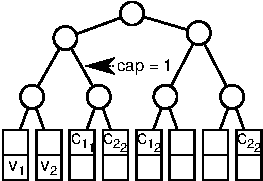
\includegraphics[width = \columnwidth]{figs/matching_no_rs}
% \caption{An example for the $\RS+\BW$ problem variant: $\achunk_{1_1}$ or $\achunk_{2_1}$ are
%located in a subtree with uplink capacity $1$. The bandwidth allocation in the right
%subtree depends on which chunk is chosen for processing in the left
%subtree.}
% \label{fig:matching_no_rs}
%\end{figure}
%
%
%\textbf{Runtime.} While \carlo{minimum weight perfect} matching problems can be
%solved in polynomial
%time~\cite{schrijver_combinatorial_optimization} using
%general algorithms, in the following, we show that for our problem
%a simple and fast greedy strategy is sufficient.
%Accordingly, we can use greedy bottom-up construction of matching.
%Its runtime is linear with respect to number of tree vertices. It is more
%efficient that more general methods of
%finding perfect matching in general bipartite graphs.
%
%\begin{corollary}
%An optimal matching of nodes to chunks can be computed greedily, by
%alternating selecting edges with the lowest cost and removing the chossen
%edge, and all edges connected to the nodes of these edge.
%\end{corollary}
%
%\begin{proof}
%Given an edge with the lowest costs, we can compute the smallest subtree, which
%contains both, the node and the chunk which are connected by the edge. Since we
%know that there is no node in a smaller subtree containing the chunk, we can
%assign the node to the chunk, and according to Lemma~\ref{lemma:local}, the
%resulting assignment will be optimal.
%\end{proof}
%
%
%
%Finally, let us observe that $\RS+\BW$ cannot be solved using this approach,
%as Lemma~\ref{lemma:uplink} does not
%hold for problem instances with $\RS$. Figure~\ref{fig:matching_no_rs}
%illustrates this problem: It shows a feasible problem instance in which, due
%to bandwidth constraints, only one chunk can be processed locally. If for
%instance $\achunk_{1_1}$ is assigned to $\VirtualNode_1$, $\achunk_{2_1}$ cannot
%be processed by $\VirtualNode_2$, since this would exceed the bandwidth
%capacity. Instead $\achunk_{2_2}$ will be processed by $\VirtualNode_2$. This
%requires bandwidth allocations on links, which would not have been utilized,
%when $\achunk_{2_1}$ would have been assigned to $\VirtualNode_1$. Hence the
%bandwidth utilization on individual links is no longer predictable in $\RS$.
%When this problem is transformed into a matching problem, the resulting
%assignment will use $\achunk_{1_1}$ and $\achunk_{2_1}$, which violates
%bandwidth constraints, although the instance itself is feasible.
%
%\textbf{Summary.}
%Figure~\ref{fig:venn_match} summarizes all problem
%variants which can be solved with our flow-based approach.
%\begin{wrapfigure}{r}{0.5\columnwidth}
%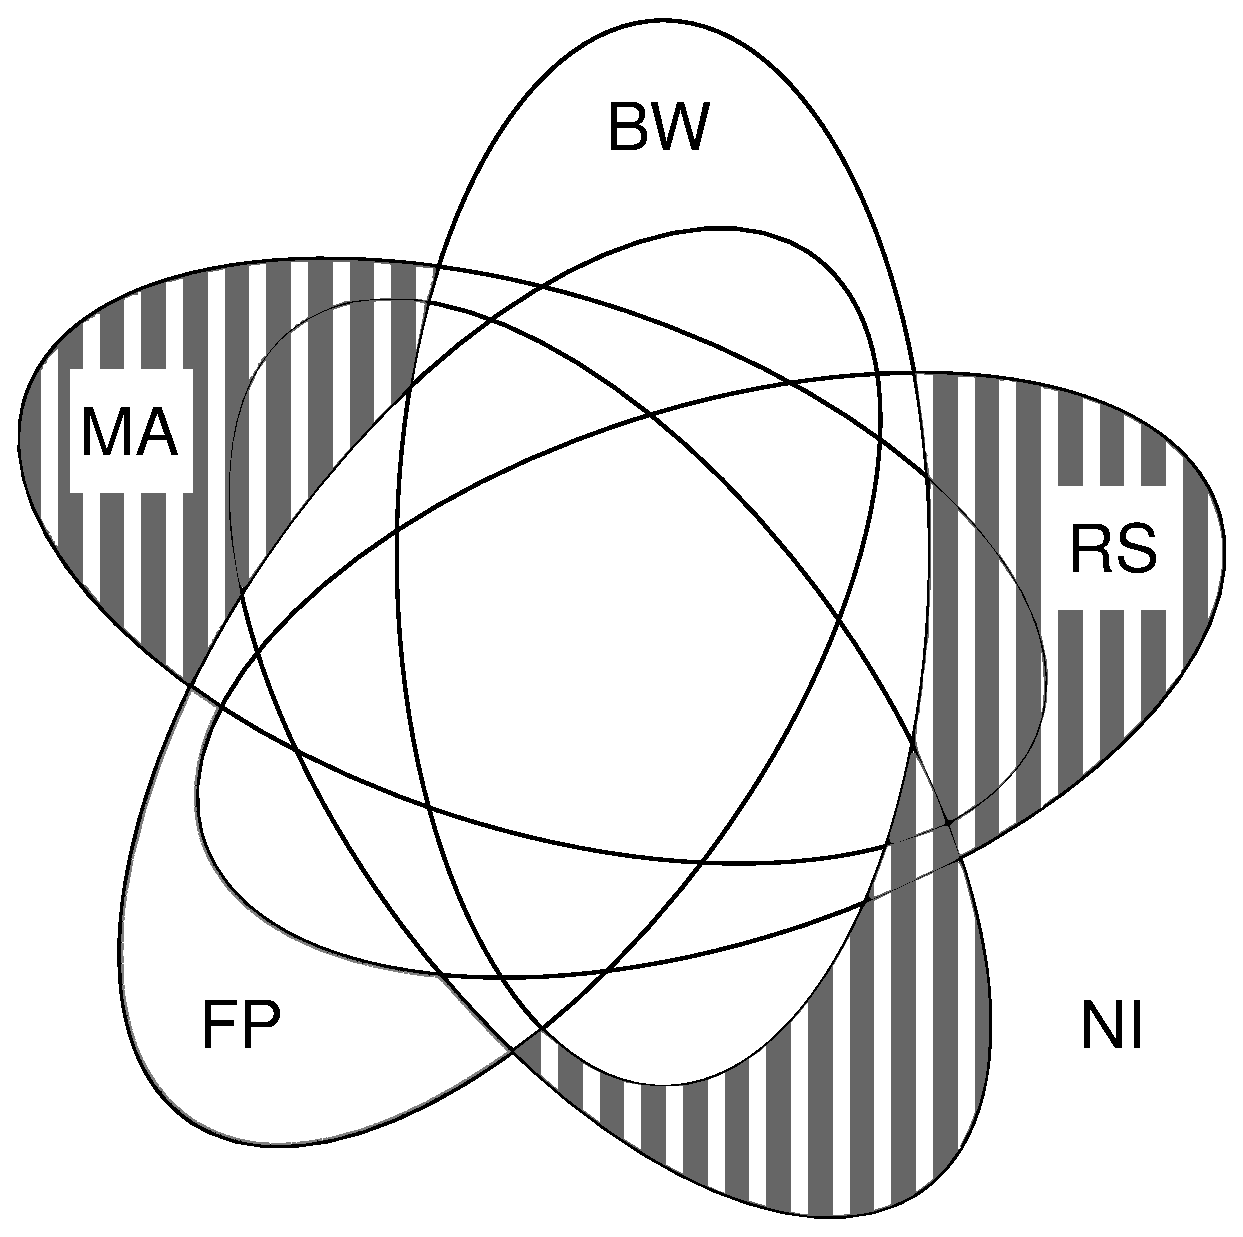
\includegraphics[width=0.48\columnwidth]{figs/venn_matching.pdf}
%\caption{Problem variants which can be solved using our matching approach.}
%\label{fig:venn_match}
%\end{wrapfigure}
%\end{comment}


\subsection{Dynamic Programming ($\FP+\CC+\MA+\BW$)}\label{ssec:dyn}

We now show that also the $\FP+\CC+\MA+\BW$ problem variant can be solved
in polynomial time.\maciek{Passive voice - consider rewrite.}
Note that this problem variant requires to find a
tradeoff between the desire to place nodes as close as possible to each other
(in order to minimize communication costs), and the desire to place nodes
as close as possible to
the chunk locations.

Figure~\ref{fig:dynamic_motivation} shows an example: one
extreme solution is to minimize the distance between chunks and nodes,
see mapping $\NodeMapping_1$ in
Figure~\ref{fig:dynamic_motivation} \emph{(left)}: the $4$ nodes are all
collocated with chunks, resulting in a zero-cost chunk access network. As a
result, the paths between the individual nodes are longer than in alternative
node placements: each node has a distance of two hops to one other node,
and four hops to two other nodes. Hence the resulting allocations for the
node interconnect sum up to $20 \cdot \CostCom$ . 
Figure~\ref{fig:dynamic_motivation} \emph{(right)} shows a different node
mapping $\NodeMapping_2$, which seeks to minimize the communication costs
between the nodes, and places all nodes in one subtree. The distance between all
nodes is two, which results in a total bandwidth allocation of $12\cdot\CostCom$
for the interconnect. However, this reduced price comes at additional costs in
the access network: $c_3$ and $c_4$ have to be transported to $v_4$ and $v_4$,
which requires a total bandwidth allocation of $8 \cdot \CostTrans$. 


\begin{figure}
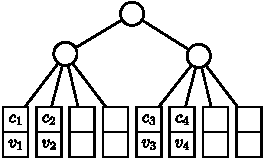
\includegraphics[width = 0.49\columnwidth]{figs/dynamic_bad}
\hfill
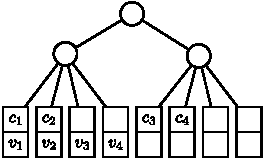
\includegraphics[width = 0.49\columnwidth]{figs/dynamic_good}
\caption{Two different node placements for the same substrate graph and chunk
locations. For $\CostTrans = \CostCom$, both solutions have an identical
footprint. In other cases, one solution outperforms the other.}
\label{fig:dynamic_motivation}
\end{figure}

\stefan{carlos figure comes here}

%\maciek{TODO: In each of previous sections we had an example where we show
%  non-triviality of the problem. Here we also have an interesting
%  example, which show that placing VMs on chunks can be arbitrarily
%  bad. In this example optimal solution places each VM in separate
%  subtree and transports every chunk to this subtree. The subtree was
%  chosen because it was able to host all the machines, unlike the
%  subtries with chunks. The reader might wonder why we considered
%  every possible location for a VM and this is exactly the reason}

Our proposed approach is based on dynamic programming, and
leverages the \emph{optimal substructure property} of $\FP+\CC+\MA+\BW$:
as we will see, optimal solutions for subproblems (namely subtrees)
can efficiently be combined into optimal solutions for larger problems.
Indeed, the $\FP+\CC+\MA+\BW$ problem
exhibits such a structure, and we show how to exploit it to
compute efficient embeddings, even in scenarios where multiple chunks
need to be assigned to flexibly placeable nodes.

\textbf{Basic ideas.} For ease of presentation, we will transform the substrate network $\Tree$
into a binary tree, using binarization:
we clone every higher-degree node,
iteratively attaching additional clones as right children
and original children as left descendants.
%Last child is placed as
%right son of last clone.

As usual in dynamic programs, we define, over the structure of the tree, an inductive formula $f$ for
the minimal cost solution \emph{given} any possible number of nodes
embedded in a given subtree. (The actual set does not matter,
due to symmetry arguments \maciek{and uplink lemma}.)
Our approach is to evaluate this function in a bottom-up
manner.
To finally compute the actual optimal embedding,
we traverse the computed minimal-cost path backwards.

Concretely, the first argument to function $f$
is a subtree $\Tree'$ (which contains a given set of chunks-in-the-subtree $\ChunkCount(\Tree')$ \maciek{We define CIS as set only to use its power later. Define it as number to avoid symbols.}),
and the
second argument is the number of nodes to be embedded in the subtree.
Function $f$ is evaluated in a bottom up manner. We initialize the
function at each leaf $\ell$, by $f(T_{\ell},x) =
\infty$ for all numbers of nodes $x$ which are larger than
the server capacity $\capacity(\ell)$;
to calculate $f(T_{\ell}, x)$, for $x \leq \capacity(\ell)$, we compute the
bandwidth allocation on the uplink of $T_{\ell}$, referred to by the function
$bw(T_{\ell},x)$: $bw(T_l,x)=  \CostTrans \cdot |x - |\ChunkCount(T_{\ell})||$ $
+ \CostCom \cdot (\Vms - x) \cdot x$,
which accounts for the bandwidth allocation on the uplink of $T_{\ell}$. The first
term represents the required bandwidth for the communication between the $x$
nodes on $\ell$, and the $\Vms - x$ nodes in the remaining parts of the substrate
network.
%Obviously the communication $x$ among the $x$ nodes within $T_l$
%does not require bandwidth on the uplink of $T_l$.
The second term represents
the bandwidth, which is necessary to transport the chunks from their location to
the node which should process the data (see Lemma~\ref{lemma:uplink} for more
details).
%Since placing nodes on servers will not require additional bandwidth
%allocations, $bw$ is equal to $f$ on all subtrees $T_l$, which consist only of
%a single leaf. If the required bandwidth $bw$ exceeds the avialble bandwidth
%$\capacity$ on the uplink, $f(T_l,x)$ is set to $\infty$, to mark the
%corresponding number of nodes in the subtree as infeasible.}

%\carlo{
After this\maciek{Remove ``this''?} initialization, we proceed to compute $f$ for non-leaf
nodes in a bottom up manner: We consider every possible split of the $x$ nodes\maciek{To split nodes into integers - rewrite.}
into two positive integer
values: we put $r$ on the right and $x - r$ on the left subtree.
That is, we take the optimal cost
(given recursively) of placing $r$ nodes in
the right subtree $\textsc{Ri}(T')$ of $T'$ and $x-r$ nodes in left subtree $\textsc{Le}(T')$ of
$T'$. Given the cheapest combination, we add the bandwidth requirements
on the uplink of $T'$ to generate the overall costs for placing $x$ nodes in $T'$.

$$f(T',x) =   \min_{r \in \{0, \ldots, x\}}  f\left(\textsc{Ri}(T'), r\right) +
f\left(\textsc{Le}(T'), x - r\right) + bw(T',x)$$

\maciek{$$f(T',x) =   \min_{0\leq r \leq x} \{  f\left(\textsc{Le}(T'), x-r\right) +
f\left(\textsc{Ri}(T'), r\right) \} + bw(T',x)$$}
Again, we set $f(T',x)$ to infinity if the required bandwidth
$bw$ exceeds the capacity $\capacity$ of the uplink of $T'$.
  
%This allocation consists of two parts: (1) The node inter-connect
%communication is easy to compute, as we know how many
%nodes are in the left and right subtree, and how many are
%outside.
%Concretely, for each node pair communicating across subtrees we
%charge $b_2 \cdot (w(e_1) +
%w(e_2))$, for each pair where one is in the subtree and the other outside,
%we charge $b_2 \cdot
%w(e_1)$. Right subtree case is symmetrical.
%(2) The chunk access cost
%can be computed by greedily matching nodes to chunks locally (first
%inside the subtree, then across subtrees, then outside $T'$).
%In particular, we can
%just consider the absolute value of the difference between the number of chunks and
%the number of nodes in a given subtree, without knowing which
%is bigger, because in our model if there are some nodes
%left, we know that some chunks from outside will use the same transfer
%as if we have excessive chunks in the subtree.

%Assume there are $c_{\ell}$ chunks in the left and $c_r$
%chunks in the right subtree. To incline minimal cost we connect chunks in
%given subtree to nodes in the same subtree. If we can no
%longer do that, because $v_i < c_i (i \in \{l,r\})$, then we connect
%leftover chunks to nodes in second subtree of $T$. If we
%can no longer do that, we connect leftover chunks outside of $T$. This
%strategy is optimal, because connecting any other way can be amended
%(TODO: need better argument here), inclining lower cost. Connections
%inside either left or right subtrees inclines cost $0$ to edges $e_1$
%and $e_2$. Connections between left and right subtree incline cost
%$b_1
%\cdot (w(e_1) + w(e_2))$. Connections from either subtree to outside
%of $T$ inclines either $b_1 \cdot w(e_1)$ or $b_2 \cdot
%w(e_2)$. Finally, we can write down our formula for $f$:


%\maciek{We will want to go through all VM placements, for each of those do greedy matching and choose the cheapest.}%
%
%\maciek{Solution for subtree - how it can look like? It is ``partial matching''. Some matched VMs and chunks, but also some chunks transported out of subtree or some %VMs/slots that will have chunks transported into from outside. So we charge already those incomplete matchings.}

%\maciek{TODO: base cases for f that take into consideration hosting
%  multiple VMs in one node}%
%
%Therefore, we have:
%\begin{eqnarray*}
%f(T', x) &=& \min_{\ell \in \{0, \ldots, x\}}  f(\textsc{Le}(T'), {\ell}) + f(\textsc{Ri}(T'), x - {\ell}) \\
%&&+ \CostTrans(\textsc{Le}(T'),{\ell},\textsc{Ri}(T'),x-l)\\ &&+ \CostCom({\ell},x-{\ell})\\
%\end{eqnarray*}
%
%\maciek{We forgot to mention how we deal with bandwidth here. Our
%  approach is to check at every placement, at every subtree whether
%  uplink edge does not exceed its capacity. If it does for any subtree, we cross out
%  this placement. We also need to show correctness of this strategy in
%  analysis - but it holds from uplink lemma.}

%\begin{comment}
%
%
%\newcommand{\SumIndex}{\ensuremath{n}}
%\begin{algorithm}[tbhp]
%\DontPrintSemicolon % Some LaTeX compilers require you to use
%%%\dontprintsemicolon instead
%\SetAlgoNoEnd
%\KwIn{$\Opt_{\SubstrateNode_l} ,
%\Opt_{\SubstrateNode_r},
%\ChunkCount_{\SubstrateNode_l},\ChunkCount_{\SubstrateNode_r} $}
%$\ChunkCount_\SubstrateNode = \ChunkCount_{\SubstrateNode_l} +
%\ChunkCount_{\SubstrateNode_r}$\;
%\For{$\SumIndex \in \{0,\dots,\Vms\}$}{
%  \For{$i \in \{0,\dots,\SumIndex\}$}{ \If{$\Opt_\SubstrateNode[\SumIndex]
%  > \Opt_{\SubstrateNode_l}[i] +
%\Opt_{\SubstrateNode_r}[\SumIndex - i]$}{
%	$\Opt_\SubstrateNode[\SumIndex] \gets \Opt_{\SubstrateNode_l}[i]
%	+
%\Opt_{\SubstrateNode_r}[\SumIndex - i]$\;
%    } }
%
% $bw \gets (\Vms -
%\SumIndex) \cdot \SumIndex \cdot \CostCom +   |i -
%\ChunkCount_\SubstrateNode| \cdot \CostTrans$\;
%  \eIf{$bw \leq \capacity(\Uplink(v))$}{
%    $\Opt_\SubstrateNode[\SumIndex] \gets \Opt_\SubstrateNode[\SumIndex]
%    + bw$\; }{ $\Opt_\SubstrateNode[\SumIndex] \gets \infty$\; } }
%%
%\caption{$aggregate(\SubstrateNode \in \SubstrateNodes)$}
%\label{algo:dynAggregation}
%\end{algorithm}
%
%List all needed functions like distance, counter of number of chunks
%in subtree.
%
%Tell how to go back through the array to reconstruct the actual
%placements. Following path of minimas. Other approach is to store pointers to minimas on lower levels as those are chosen.
%
%(Base case) We fill the entire array $Opt_l$ for the leaf $l$ with zeros. It means that we allow hosting $0, 1, \ldots, n$ VMs in this leaf. We can restrict the number of VMs that are hosted in the same leaf by some constant $x$ (that can be independent for every leaf) by setting $Opt_l[x+1] = Opt_l[x+2] = \ldots = Opt_l[n] = \infty$.
%
%\end{comment}


\textbf{Analysis.}
The correctness and optimality of our dynamic program
is due to the decoupling of the costs induced by the tree
structure of $\Tree$ and the  substructure
optimality property.
The substructure optimality follows from the observation that
costs can be accounted on the uplink\maciek{Passive voice - consider rewrite.}
, and the fact
 that we check each possible node distribution.
For each substrate vertex ($n_S$ many) we have
to check the cost of all possible splits,
resulting in an overall complexity of $\mathcal{O}(n_S \cdot n_V^2)$.
The runtime to binarize $\Tree$ is asymptotically negligible.

%\textbf{Summary.}
%Figure~\ref{fig:venn_dp} summarizes all problem
%variants which can be solved with our dynamic programming approach.
%\begin{wrapfigure}{r}{0.5\columnwidth}
%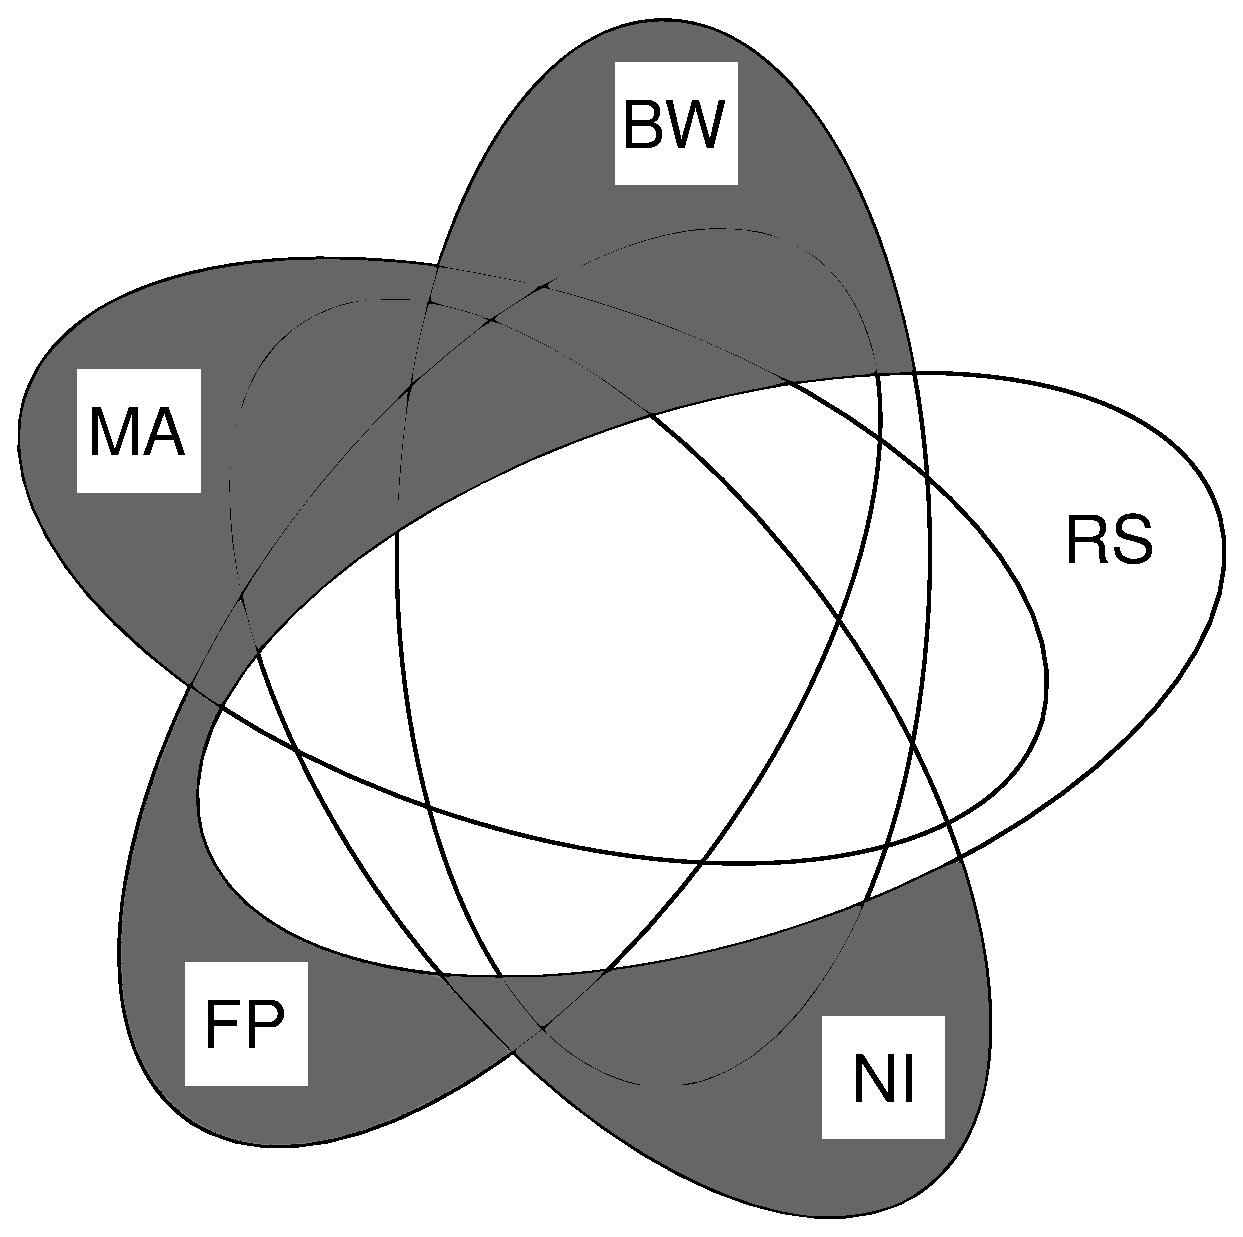
\includegraphics[width=0.48\columnwidth]{figs/venn_dp.pdf}
%\caption{Variants solved by programming approach.}
%\label{fig:venn_dp}
%\end{wrapfigure}

\subsection{Remark: Simple Problems}

To conclude, for the sake of completeness, we also observe that there are
several problems which
allow for a trivial solution. Concretely, problems with $\FP$
plus any combination of
$\RS$ and $\BW$ (but without $\CC$ or $\MA$) can easily be solved by mapping nodes to chunk locations.
%Figure~\ref{fig:venn_trivial}
%shows a Venn diagram of the trivial property combinations.

\begin{wrapfigure}{r}{0.5\columnwidth}
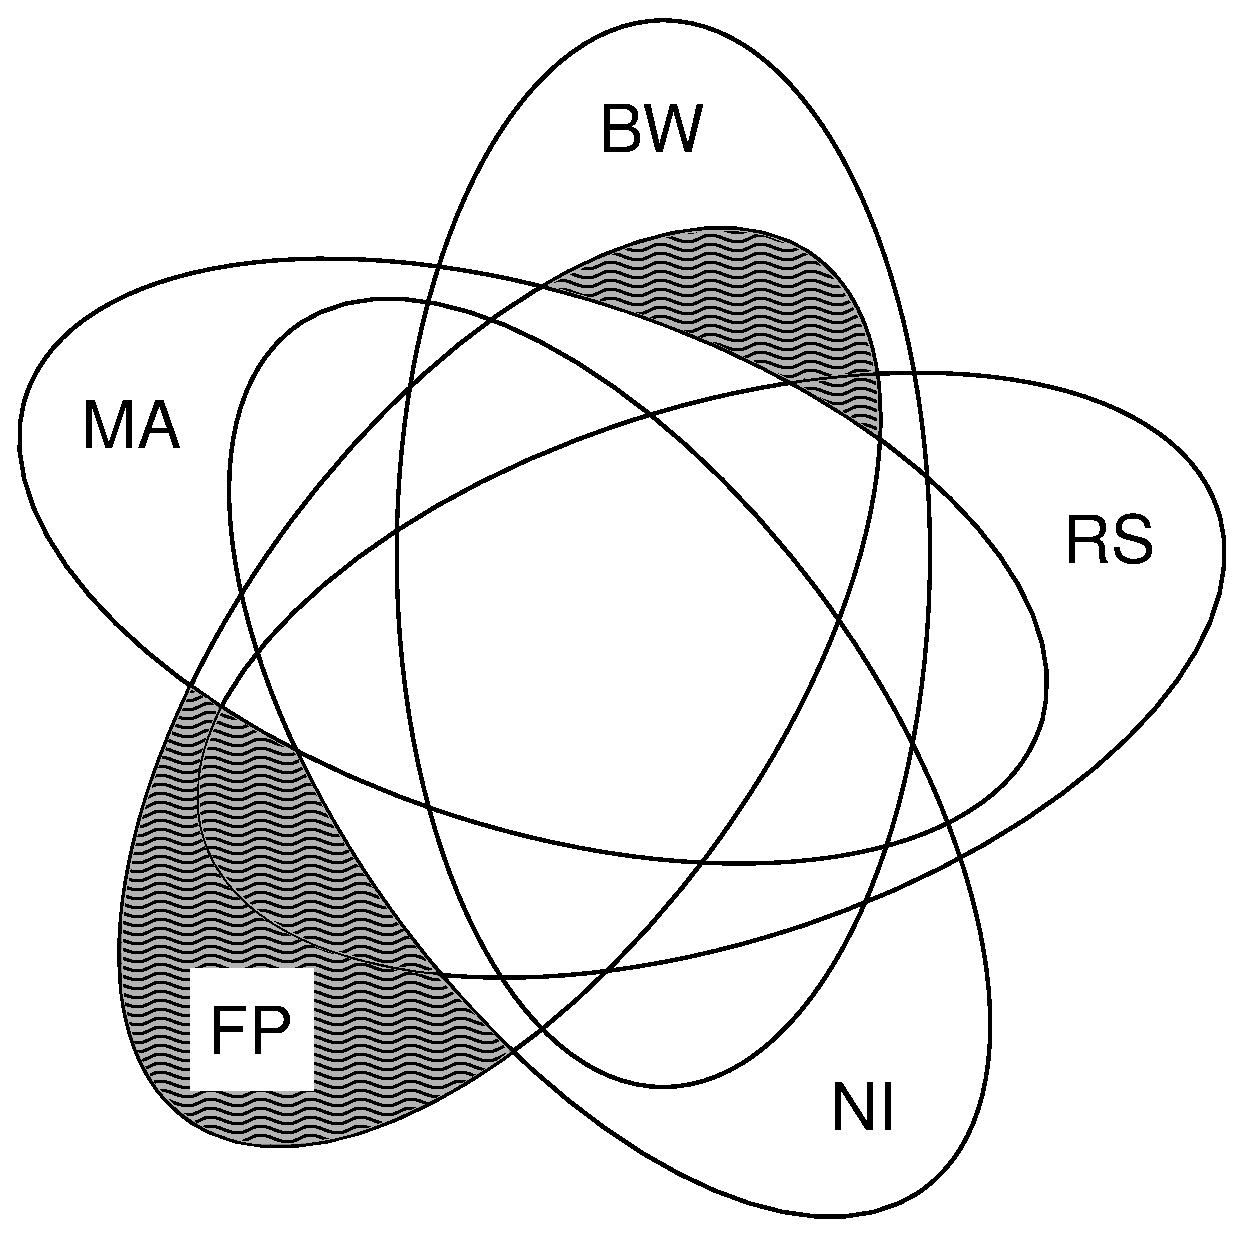
\includegraphics[width=0.48\columnwidth]{figs/venn_trivial.pdf}
\caption{Trivially solvable problem variants.}
\label{fig:venn_trivial}
\end{wrapfigure}

%%%%%%%%%%%%%%%%%%%%%%%%%%%%%%%%%%%%%
\section{NP-Hardness Results}\label{sec:np}

%\carlo{TODO: Move embedd in surrounding text / move. Figure~\ref{fig:venn_full}
%gives an overview of the problems, which have been solved in polynomial time in
%Section~\ref{sec:poly}. This section will present proofs to show that all
%remaining property combinations (marked in black) are np-hard.}

We have seen that even problems with multiple dimensions of
flexibility can be solved optimally in polynomial time\maciek{Passive voice - consider rewrite.}
.
This section now points out fundamental
limitations in terms of computational tractability. In particular, we
will show that problems become NP-hard if multiple chunks have to be
assigned to a flexibly placeable node ($\FP+\RS+\MA$ is proved NP-hard in
Section~\ref{ssec:fprsma}), and if inter-connects have to be established
between flexible nodes ($\FP+\RS+\CC$ is proved NP-hard in Section~\ref{ssec:fprscc}); both
results hold even in uncapacitated networks, and even in small-diameter
substrate networks (namely two- or three-level trees~\cite{fattree}).
The hardness of $\FP+\RS+\MA$ and $\FP+\RS+\CC$ imply
the hardness of four additional, more general models, as
summarized in the following figure: \maciek{TODO: reference the figure, add caption.}

\begin{figure}[htbp]
\small
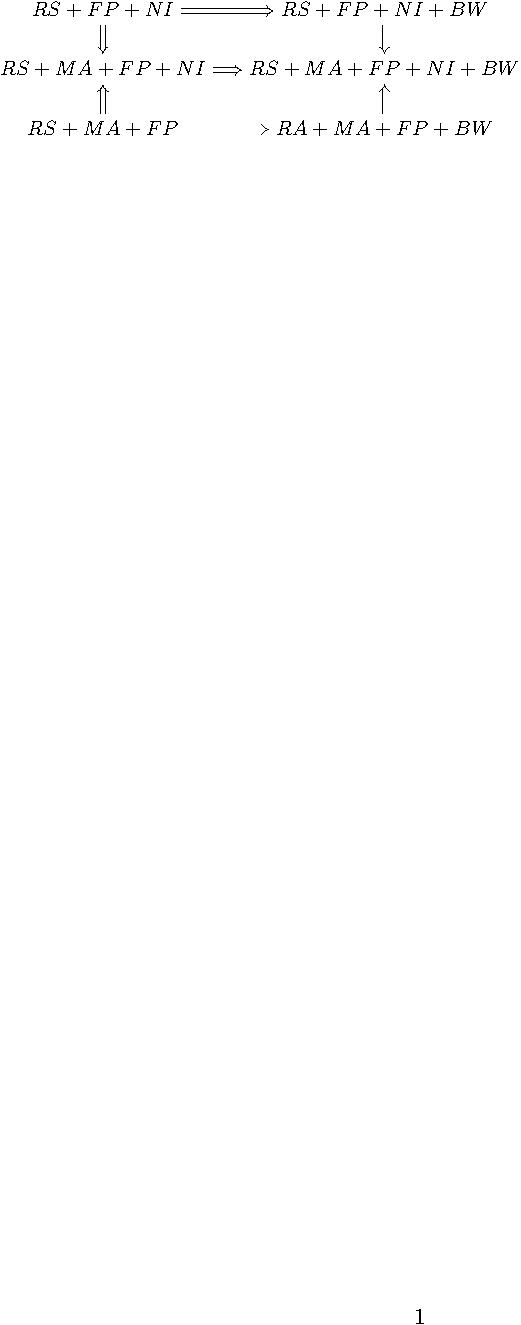
\includegraphics[width = \columnwidth]{figs/np_implications}
% \begin{tikzcd}[arrows=Rightarrow, column sep = 0.5cm, row sep = 0.5cm]
%RS+FP+NI\arrow{r}{}\arrow{d}{}& RS+FP+NI+BW\arrow{d}{}\\
%% RS+FP+NI\arrow{ur}{}\arrow{dr}\\
%RS+MA+FP+NI\arrow{r}{}&RS+MA+FP+NI+BW\\
%RS+MA+FP\arrow{r}{}\arrow{u}&RA+MA+FP+BW\arrow{u}{}\\
%\end{tikzcd}
\end{figure}

Additional NP-hardness results appear in the Appendix.

\subsection{Introduction to 3D Perfect Matching}

Both the hardness of $\FP+\RS+\MA$ and $\FP+\RS+\CC$ are shown by a reduction
from the NP-complete problem of \emph{3D Perfect Matching}~\cite{3dmatch},
which
can be seen as a generalization of bipartite matchings to 3-uniform
hypergraphs\maciek{Passive voice - consider rewrite.}
. We will refer to this problem by $\TDM$, and for completeness,
review it in the following.

$\TDM$ is defined as follows. We are given three finite and disjoint
sets $X$, $Y$, and $Z$ of cardinality $k$, as well as a subset of triples $T\subset
X \times Y \times Z$.  Set $M \subseteq T$ is a 3-dimensional matching
if and only if, for any two distinct triples $t_1=(x_1, y_1, z_1) \in M$
and $t_2=(x_2, y_2, z_2) \in M$, it holds that $x_1\neq x_2$, $y_1\neq
y_2$, and $z_1\neq z_2$. Our goal is to decide if we can construct
a $M \subseteq T$ which is \emph{perfect}, that is, a subset which covers all
elements of $X \times Y \times Z$.

\maciek{Our goal is to decide if we can construct
a $M \subseteq T$ which is \emph{perfect}, that is, a subset which covers all
elements of $X \times Y \times Z$ exactly once. }

%TODO: image like this: \url{https://upload.wikimedia.org/wikipedia/commons/thumb/5/50/3-dimensional-matching.svg/240px-3-dimensional-matching.svg.png}

\subsection{Multi-Assignments are hard ($\FP+\RS+\MA$)}\label{ssec:fprsma}

Our proof that $\FP+\RS+\MA$ is NP-hard is based on the following main ideas.
We encode a $\TDM$ instance as an $\FP+\RS+\MA$ instance as follows:\maciek{Those basic ideas are shared between two proofs. Maybe we should put those in the intro? But it is good the way it is also.}

 \begin{itemize}
 \item For every element in the universe $X\cup Y\cup
 Z$, we create a chunk type. Intuitively, in $\TDM$,
 each element must be covered, which corresponds to the requirement
 of $\FP+\RS+\MA$,
 that each chunk type is processed.

 \item We will encode each triple as three leaves \maciek{Gadget with three leaves instead of just three leaves} in
 a substrate tree $\Tree$. The three leaves are close to each
 other in $\Tree$, and the placement of chunk replicas in $\FP+\RS+\MA$
 corresponds to the elements of the
 triples in these leaves.

 \item The node placement will correspond to choice of triples,
 independently in which leaf the node is mapped.
 A node will process the chunk which is located on the same server \maciek{Notation of ``the same server'' can be ambigous},
 as well as the chunks in other two leaves of the same gadget.

\item In order to turn the optimization problem into a decision problem, we will use
a cost threshold $\Thr$; solutions of higher costs are considered infeasible. \maciek{Setting threshold this way prevents transportation of chunks between gadgets.}

\end{itemize}


\textbf{Construction.}
Given an instance $I$ of $\TDM$ \maciek{we might want to set $k$ to be $k$ from this instance, because later we use this $k$ and the reader might have hard time finding which $k$ are we talking about}, we construct an instance $I'$ of
$\FP+\RS+\MA$ as follows:
\begin{itemize}
\item \emph{Tree Construction:} We create a tree consisting of a root,
and for each triple, we create a gadget which we directly attach as
child of the root. The gadget is of height 2,
and has the following form:
The gadget of each triple $t_i$ consists of an inner node (a router) and three leaves.
\item \emph{Chunks and chunk replicas:} For each element in $X$, $Y$ and $Z$,
 we create a chunk type
($3 \cdot k$ in total \maciek{This can be alternative place where we tell that $k$ is from the instance}). Every gadget
contains three chunk replicas, corresponding to the elements of $t_i$.
\item \emph{Other properties:} We set the number of to-be-embedded nodes to $k$,
$\CostTrans$ to $1$, and the number of chunk slots in each node to the multi-assignment factor
$\MaFactor=3$.
%\stefan{what
%is the number of slots here?}\maciek{it is number of replicas that
%each VM can process (the MA property)}.
We use a threshold $\Thr= 4
\cdot k$.
% \maciek{If we update the model to take care of hosting
%  multiple VMs in one leaf, we should set this instance to allow only
%  one VM per leaf. However, any number of VMs per leaf will be OK for
%  this proof.}
\end{itemize}

\textbf{Example.} Figure~\ref{fig:fprsma} shows an example of our construction: An
instance $I$ of 3-DM is given: The disjoint sets $X$, $Y$ and $Z$ have a
cardinality $k=2$. We will refer to the two elements in $X$ as $x_1$ and $x_2$,
and use the same notation for the other two sets. $T$ contains the three triples
$(x_1, y_1,
z_1)$, $(x_2, y_1, z_2)$, and $(x_2, y_2, z_2)$. The goal of 3-DM is to find a
subset $M \subseteq T$, which contains each element in each of the three sets
exactly once. For this instance the only solution is $M =
\{(x_1,y_1,z_1),(x_2,y_2,z_2))\}$.

To construct the corresponding instance $I'$ of $\FP+\RS+\MA$, we
create a gadget for each triple in $T$. The gadgets contain a chunk  the
type of the variable, for each variable that occurs in the triple. The triple
$(x_2, y_1, z_2)$ of the instance is represented by the middle gadget in
Figure~\ref{fig:fprsma}. The objective of $I'$ is to spawn $k=2$ nodes,
with the smallest possible footprint. If the total footprint is $\leq
2\cdot2\cdot k$, we can construct a solution to $I$ from the solution to $I'$.
The footprint consists of the costs which occur when a node is embedded in a
gadget, and the three chunks of that gadget which are assigned to that node: one of
the chunks is collocated with the node, the other two have to be transferred
via two hops, inflicting costs $1$ on each hop.
%\begin{figure}[htbp]
%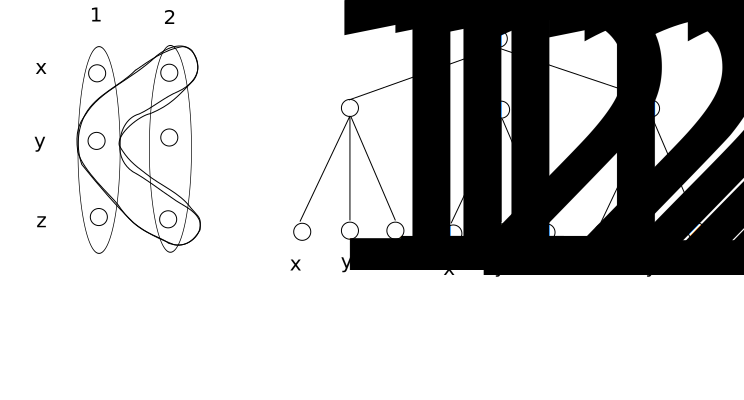
\includegraphics[width = \columnwidth]{figs/example-matching}
%\end{figure}
\begin{figure}[t]
\includegraphics[width = 0.3\columnwidth]{figs/np_3dm_formular}
\hfill
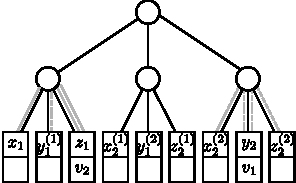
\includegraphics[width = 0.6\columnwidth]{figs/np_3dm_construction}
\caption{\textit{Left:} A $\TDM$ instance with three triples:
$(x_1, y_1, z_1)$, $(x_2, y_1, z_2)$, and $(x_2, y_2, z_2)$. The solution is
indicated by the grey triples; the dashed triple is not used for the
solution. \textit{Right:} The corresponding problem and solution of $\FP + \MA
+ \RS$.}
\label{fig:fprsma}
\end{figure}


\textbf{Correctness.}
Given these concepts, we can now show the computational hardness.
\begin{theorem}
$\FP+\RS+\MA$ is NP-hard.
\end{theorem}
\begin{proof}
Let $I$ be an instance of $\TDM$ and let $I'$ be an instance of
$\FP+\RS+\MA$ constructed as described above.
We prove that $I'$ has solution of cost $\leq \Thr$ if ($\Rightarrow$) and only if
($\Leftarrow$)
$I$ has a matching of size $k$.

($\Rightarrow$) Let us take a solution to $\TDM$. We place a node in every
gadget that corresponds to the chosen triples. We match every chunk in a
gadget to a node in this gadget (only the chosen ones \maciek{I do not understand ``only the chosen ones''}). This solution has
cost exactly $\Thr$. As every element of the universe is covered, every
chunk type is processed.

($\Leftarrow$) Let us take a solution to $\FP+\RS+\MA$ of cost $\leq \Thr$. We
choose triples that correspond to gadgets where there are nodes. Since
all chunks are processed, every element of $X$, $Y$ and $Z$ is matched. Each
node must processes chunks that corresponds to the triple, otherwise the
cost must be larger than $\Thr$ (high costs for the connection between
nodes and chunks \maciek{high costs for chunk transportation}).
\end{proof}


\subsection{Inter-connects are hard ($\FP+\RS+\CC$)}\label{ssec:fprscc}


Next, we prove that the joint optimization of node placement and replica selection
is NP-hard if an inter-connect has to be established between nodes.
In our terminology, this is the $\FP+\RS+\CC$ problem.

\maciek{At least one sentence of introduction should belong here. We will modify the previous proof, we will use the ``sticking together'' property of quadratic communication function.}
  
\textbf{Construction.}
Let $I$ be an instance of $\TDM$. We will create an instance $I'$
for $\FP+\RS+\CC$ as follows:
\begin{itemize}
\item We will construct the same tree as in previous reduction with
chunk replicas placed in the same way.
\item The communication cost in the inter-connect is set to $\CostCom = 1$.
\item The number of nodes (virtual machines) is $\Vms = 3 \cdot k$, where $k$ is the set cardinality.
\item We use a threshold $\Thr =  6 \cdot k + 18 \cdot 
(k - 1) \cdot k$.\maciek{$\Thr = 18 \cdot k^2 - 12 \cdot k$. The threshold is designed to be communication cost of $3\cdot k$ VMs embedded in leaves of tree consisting of $k$ gadgets (no chunks).}
%\maciek{If we update the model to take care of hosting
%  multiple VMs in one leaf, we should set this instance to allow only
%  one VM per leaf. In this proof it also does not matter, as it is
%  already forced by infinite transportation cost, however we need to
%  define it anyway.
%  }
\item We set the access cost $\CostTrans$ to a chunk replica to a high value $W$. This will force
nodes to be collocated with the replica. One example of sufficient
(and polynomial but minimal) $W$
is the value of the threshold $\Thr$ defined above. Every solution that does not match chunks to VMs those are sitting on top of never has cost $\leq \Thr$, because it inflicts cost of $W=\Thr$ over every link it transports the chunk.

\maciek{One example of sufficient
(and polynomial but perhaps not minimal) $W$
is the value of the threshold $\Thr+1$ defined above. Every solution that does not match chunks to VMs those are sitting on top of never has cost $\geq \Thr$, because it inflicts cost of $W=\Thr+1$ over every link it transports the chunk.}


\end{itemize}

We again focus on instances with unit server capacities.

\textbf{Proof of correctness.}
Intuitively, in order to minimize embedding costs,
nodes should be placed on near-by replicas. We use the following
helper lemma.
\begin{lemma}\label{lemma:helper}
In every valid solution of $I'$ of cost $\leq \Thr$, each gadget
falls in one of two categories:
$k$ gadgets have exactly
$3$ nodes, and $n-k$ gadgets remain empty.
\end{lemma}
\begin{proof}
Since $W$ is large enough, nodes will always be placed
directly on chunks (the access network cost is zero).
Moreover, since
is valid, $3 \cdot k$ nodes are mapped
directly to the different chunk locations.
Now, consider any pair of nodes communicating over the
inter-connect; due to our construction, the communication cost
for each such pair is either
2 hops (if they belong to the same gadget) or 4 hops (if they belong
to different gadgets).
The lemma then follows from the observation that $\Thr$
is chosen such that it is never possible to distribute nodes
among more than $k$ gadgets.
\end{proof}

\begin{theorem}
$\FP+\RS+\CC$ is NP-hard.
\end{theorem}
\begin{proof}
Let $I$ be an instance of $\TDM$ and let $I'$ be an instance of
$\FP+\RS+\CC$ constructed as described above.
We prove that $I'$ has solution of cost $\leq \Thr$ if ($\Rightarrow$) and only if
($\Leftarrow$)
$I$ has a solution.

($\Rightarrow$) In order to compute a solution
for $I'$ given a solution for $I$, we proceed as follows.
Given a covering set\maciek{an exact covering set} of triples $S = \{t_1, t_2, \ldots, t_k\}$, we place three nodes in each gadget that
corresponds to every triple of $S$. Chunks are matched to nodes that are located
on the same server.

The solution has the following cost:
(1) the communication cost inside a gadget is $2 \cdot {3 \choose 2}$,
  as every pair contributes two hops;
  (2) the communication cost from each gadget to all other gadgets is $4
  \cdot 3 \cdot 3 \cdot (k - 1) / 2$, where the factor $4$ is
  for the
  communication over $4$ hops, the factor $3$
  corresponds to the number of nodes per gadget, and
  $3 \cdot (k-1)$ is the number of nodes in remote gadgets;
  as we count each pair twice, we need to divide by two in the end.
Summing up over all $k$ gadgets, we get exactly $\Thr$.

($\Leftarrow$) Given a solution for $I'$,
we can exploit Lemma~\ref{lemma:helper} to construct a solution for $I$.
We know that in any solution of cost at most $\Thr$,
$k$ gadgets contain exactly 3 nodes. These gadgets correspond to a valid
3D Perfect Matching: every
chunk was processed and hence every element in the $X \cup Y \cup Z$ is covered. \maciek{every chunk type has its exactly one replica processed and hence every element is covered exactly once.}
\end{proof}

Finally, let us conclude by remarking that all NP-hard problems discussed in this paper
are obviously also in NP (and hence NP-complete): solutions can be verified efficiently.

%%%%%%%%%%%%%%%%%%%%%%%%%%%%%%%%%%%%%
\section{Related Work}\label{sec:relwork}

There has recently been much interest in programming models and distributed
system architectures for the processing and analysis of big data (e.g.~\cite{nodb,mapreduce,shark}). The model studied in
this paper is motivated by MapReduce~\cite{mapreduce} like batch-processing applications, also known
from the popular open-source implementation \emph{Apache Hadoop}.
These applications
generate large amounts of network traffic~\cite{orchestra,talk-about,amazonbw},
and over the last years, several systems have been proposed which provide
a provable network performance, also in shared cloud environments, by supporting explicit
relative~\cite{faircloud,elasticswitch,seawall}
or, as in the case of our paper, \emph{absolute}~\cite{oktopus,secondnet,drl,gatekeeper,proteus} bandwidth reservations
between the virtual machines.
In particular, the notion of virtual networks which combine compute and network resources has been introduced.
For a good survey on network virtualization and in particular virtual network embeddings,
we refer the reader to~\cite{boutaba-survey} and~\cite{fischer-survey}.

The most popular virtual network abstraction for batch-processing applications today is the \emph{virtual cluster},
introduced in the Oktopus paper~\cite{oktopus}, and later studied by many others~\cite{talk-about,proteus}.
Several heuristics have been developed to compute ``good'' embeddings of virtual clusters: embeddings
with small footprints (minimal bandwidth reservation costs).~\cite{oktopus,talk-about,proteus}
The virtual network embedding problem has also been studied for more general graph abstractions
(e.g., motivated by wide-area networks).~\cite{infocom2009,ammar,turner,simannealing,ucc12mip,zhu06}

From a theoretical perspective, the virtual network embedding problem can be seen as a generalization
of classic VPN graph embedding problems~\cite{Goyal2008,gupta2001provisioning},
in the sense that in virtual network embedding problems, also the embedding endpoints are flexible and subject to optimization.
In this sense, the virtual network embedding problem can also be seen as a generalization of the
classic NP-hard Minimum Linear Arrangement problem which asks for the
embedding of guest graphs on a simple \emph{line topology} (rather than tree-like topologies as
studied in this paper).~\cite{mla,mla-survey}
There exist several interesting algorithms for the Minimum Linear Arrangement problem,
e.g., providing sublogarithmic approximation ratios~\cite{mla-feige}.

However, to the best of our knowledge, we are the first to provide an algorithmic
study of the virtual cluster embedding problem which takes into account
data locality as well as the possibility to select replicas. As we have shown in this paper,
the resulting problems can be seen as interesting new variants of several classic optimization
problems, such as hitting set and 3-dimensional matching problems~\cite{3SC-hard} as well as flow problems~\cite{korte2002combinatorial}.

%%%%%%%%%%%%%%%%%%%%%%%%%%%%%%%%%%%%%
\section{Summary and Conclusion}\label{sec:conclusion}

This paper investigated data data locality aware algorithms which exploit two fundamental
degrees of freedom in virtual cluster
embedding problems: replica selection and flexible node placement. In order to
chart the landscape of the problem complexity, we
decomposed the problem into its fundamental aspects,
namely $\RS$, $\MA$, $\FP$, $\CC$, and $\BW$, and studied the computational
tractability of different combinations.

In particular, we have shown that
at the heart of our model lie interesting new variants of classic
optimization problems related to matchings and flows. Interestingly, despite the
different dimensions of flexibility (in terms of replica selection, assignment and embedding),
many problem instances can actually be solved in polynomial time.
On the negative side, we have also shown that there exist computationally hard
problems even in uncapacitated networks. In particular,
we have shown that several embeddings problems are NP-hard already in two- and three-level trees
(a practically relevant result given today's datacenter topologies~\cite{fattree}),
and even if the the number of replicas is bounded by two.
\begin{table}


\begin{small}
\begin{tabular}{|l|l|p{4cm}|}
\hline
\multirow{3}{*}{NP-hard} & 5 combinations & \mbox{$\RS+\MA+\FP+\CC+\BW$}\\
\cline{2-3}
 & 4 combinations &  \mbox{$\RS+\MA+\FP+\CC$}; \mbox{$\RS+\MA+\FP+\BW$};
\mbox{$\RS+\FP+\CC+\BW$} \\ \cline{2-3}
 & 3 combinations &\mbox{$\RS+\MA+\FP$}; \mbox{$\RS+\FP+\CC$} \\
 \hline
 \hline
\multirow{3}{*}{Flow} & 4 combinations & \mbox{$\RS+\MA+\CC+\BW$} \\ \cline{2-3}
 & 3 combinations & \mbox{$\RS+\CC+\BW$}; \mbox{$\RS+\MA+\BW$}    \\ \cline{2-3}
 & 2 combinations &$\RS+\BW$ \\
 \hline
 \hline
\multirow{3}{*}{DP} & 4 combinations & \mbox{$\MA+\FP+\CC+\BW$} \\ \cline{2-3}
 & 3 combinations &   \mbox{$\MA+\FP+\CC$};
\mbox{$\MA+\FP+\BW$}; \mbox{$\FP+\CC+\BW$} \\ \cline{2-3}
 & 2 combinations &\mbox{$\MA+\FP$}; \mbox{$\FP+\CC$};
\mbox{$\FP+\BW$} \\
 \hline
 \hline
\multirow{3}{*}{Matching} &3 combinations&
\mbox{$\RS+\MA+\CC$}; \mbox{$\MA+\CC+\BW$}  \\
\cline{2-3}
 & 2 combinations & \mbox{$\RS+\MA$};
\mbox{$\RS+\CC$}; \mbox{$\MA+\CC$};
\mbox{$\MA+\BW$}; \mbox{$\CC+\BW$} \\ \cline{2-3}
& 1 combinations & \mbox{$\RS$}; \mbox{$\MA$};
\mbox{$\CC$}; \mbox{$\BW$}\\
 \hline
 \hline
 \multirow{3}{*}{0 Cost} & 3 combinations & \mbox{$\RS+\FP+\BW$}\\
\cline{2-3}
 & 2 combinations & \mbox{$\RS+\FP$}; \mbox{$\FP+\BW$}
\\ \cline{2-3}
 & 1 combinations & \mbox{$\FP$}\\
 \hline
\end{tabular}
\end{small}
\caption{
The use cases of the proposed algorithms, expressed in property
combinations which it can solve faster, than any other algorithm.
\maciek{Visual side of this table - cell padding, FP+NI aligned to right; there is place for saying dynamic programming instead of DP.}
}
\label{tab:summary}
\end{table}


Our results are summarized in
Figure~\ref{tab:summary}.
One interesting takeaway from this figure regards
the question which properties render the problem
NP-hard. For instance, we see that interestingly, $\BW$
does not influence the hardness of any problem variant,
while $\RS$ is crucial for NP-hardness.
$\MA$ only affects hardness if combined with $\RS$.
$\CC$ is trivial without $\FP$, and $\FP$ requires
more sophisticated algorithms when combined with $\CC$ or $\MA$;
in combination with $\RS$ and $\MA$ or $\CC$, $\FP$ renders the
problem NP-hard.

%\begin{figure}
%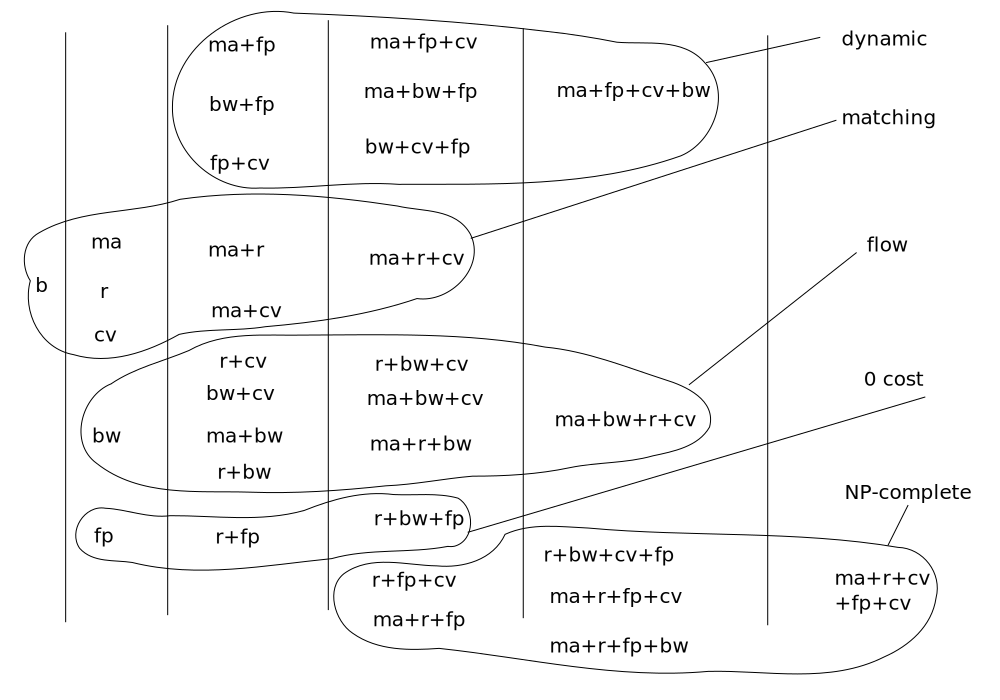
\includegraphics[width=\columnwidth]{figs/summary}
%\caption{\maciek{This figure is wrong in couple places, but I sent you an e-mail what should be redone.}Summary of results. As this paper only presented algorithms %(approaches indicated in the same
%color and pattern as in the previous figures) for the most
%difficult problems and, respectively, proved NP-hardness (indicated in black) of the simplest
%problems, several additional results are simple implications. In this figure,
%we always suggest the best (simplest and fastest) approach to solve a specific problem variant.}
%\label{fig:summary}
%\end{figure}


%\begin{figure}[t]
%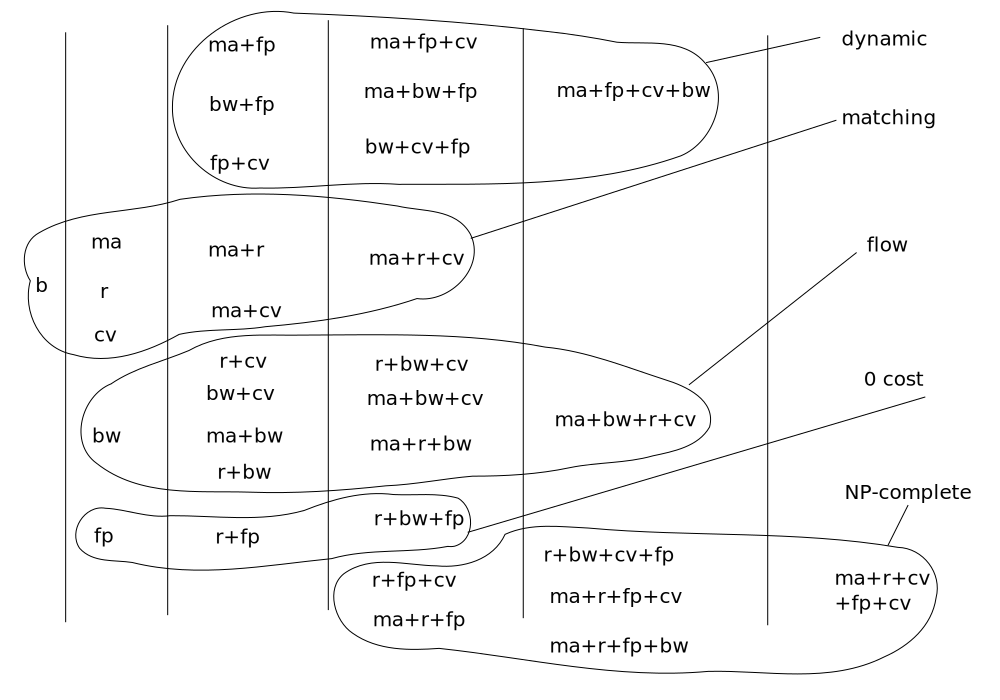
\includegraphics[width = \columnwidth]{figs/summary}
%\caption{Summary of results. As this paper only presented algorithms for the most
%difficult problems and, respectively, proved NP-hardness of the simplest
%problems, several additional results are simple implications (indicated by arrows).}
%\label{fig:summary}
%\end{figure}


Our paper draws a complete picture of what can and cannot be
computed optimally in our setting, and may be of interest both to the algorithm
and the networking community. At the same time, we understand our model and work
as a first step, and believe that our paper opens several interesting
questions for future research, for instance, regarding randomized
or approximation algorithms.


%%%%%%%%%%%%%%%%%%%%%%%%%%%%%%%%%%%%%
%\bibliographystyle{alpha}
\bibliographystyle{abbrv}
\bibliography{references}

%%%%%%%%%%%%%%%%%%%%%%%%%%%%%%%%%%%%%
\begin{appendix}

%\begin{comment}

\section{Replica selection is hard}\label{ap:tworep}

We have seen that replica selection flexibilities can render problems computationally hard.
In the following, we will explore the minimal requirements for rendering replica selection hard.
In particular, we will show that already two replicas for each chunk type are sufficient to
introduce intractability.

In the following, we allow the number of chunk types to be smaller than the number of nodes.
 The ``idle'' nodes however do participate in the inter-connect communication (in practical terms: in the shuffle phase
 and the reducing phase).
% (Note that the dynamic algorithms presented above work for this model too.)

%they do not necessarily have to We need to introduce the idle machines extension, that is
%  needed for reduction to work. Motivation: We can say that idle vms are only idle in
%  mapping phase of MapReduce, but participate in shuffle phase. We can
%  call it ``Additional shuffle nodes extension''.We can also tell the reader that our
%  dynamic program works for this extension (f(T,x,idle)) . Considering
%  mixing this extension with $\MA$:
%   (1) NP-hardness
%  proofs holds with setting $idle=0$; (2) dynamic program work with
%  assumption that every VM either processes 0 chunks or processes
%  maximum number of chunks (3) our flow algorithm
%  work with contrary model assumption, that we can have arbitrary
%  number of chunks assigned to VMs. }

%\maciek{We need to tell the reader that our proof holds only for
%  (NP-complete) subset of 3SAT where we have more than 4
%  clauses. Otherwise the bandwidth lemma does not work!}

In the following, we first give an alternative proof for the hardness of $\CC+\FP+\RS+\BW$.
Subsequently, we show that the 2-replica variant $\RS(2)$ is hard.

%For our proof, we assume a model where there can be more nodes than chunk types,
%and additional nodes only participate in the inter-connect, and not the replica access network.

% TODO
%\subsection{Three replicas are hard ($\CC+\FP+\RS+\BW$)}\label{ssec:three}

We prove that $\CC+\RS+\FP+\BW$ is NP-hard by reduction from the \emph{Boolean Satisfiability Problem} ($\SAT$).
Since $\SAT$ is a decision
problem, we 
introduce a cost threshold $\Thr$ to transform $\CC+\RS+\FP+\BW$ into a decision problem too.

Let's first recall that the $\SAT$ problem asks whether a positive valuation exists
for a formula $\Formula$ with $\clauses$ clauses and $\variables$ variables.
In the following, we will only focus on $\SAT$ instances of at least four variables;
this $\SAT$ variant is still NP-hard.

\textbf{Construction.}
Given any formula $\Formula$ in \emph{Conjunctive Normal Form (CNF)} with at least four variables, we produce
a $\RS+\FP+\BW$ instance as follows. First, we construct a substrate tree $\Tree_{\Formula}$, consisting of
a root and separate gadgets for each variable of $\Formula$, each of which
is a child of the root.
The gadget of variable $\variab$ consists of $\aroot(\variab)$ and its two children:
$\positive(\variab)$ and $\negative(\variab)$. Child $\positive(\variab)$ has $\clauses$
many children \maciek{labeled (we don't want to give the impression that there are chunks named this way)} $\nu_1, \nu_2, \ldots, \nu_{\clauses}$, and child
$\negative(\variab)$ has
$\clauses$ many children \maciek{labeled} $\neg \nu_1, \neg \nu_2, \dots, \nu_{\clauses}$. Every
gadget has the same structure: the same height and the same number of
leaves. This construction is illustrated in
Table~\ref{fig:construction_3sat}.


\begin{figure}
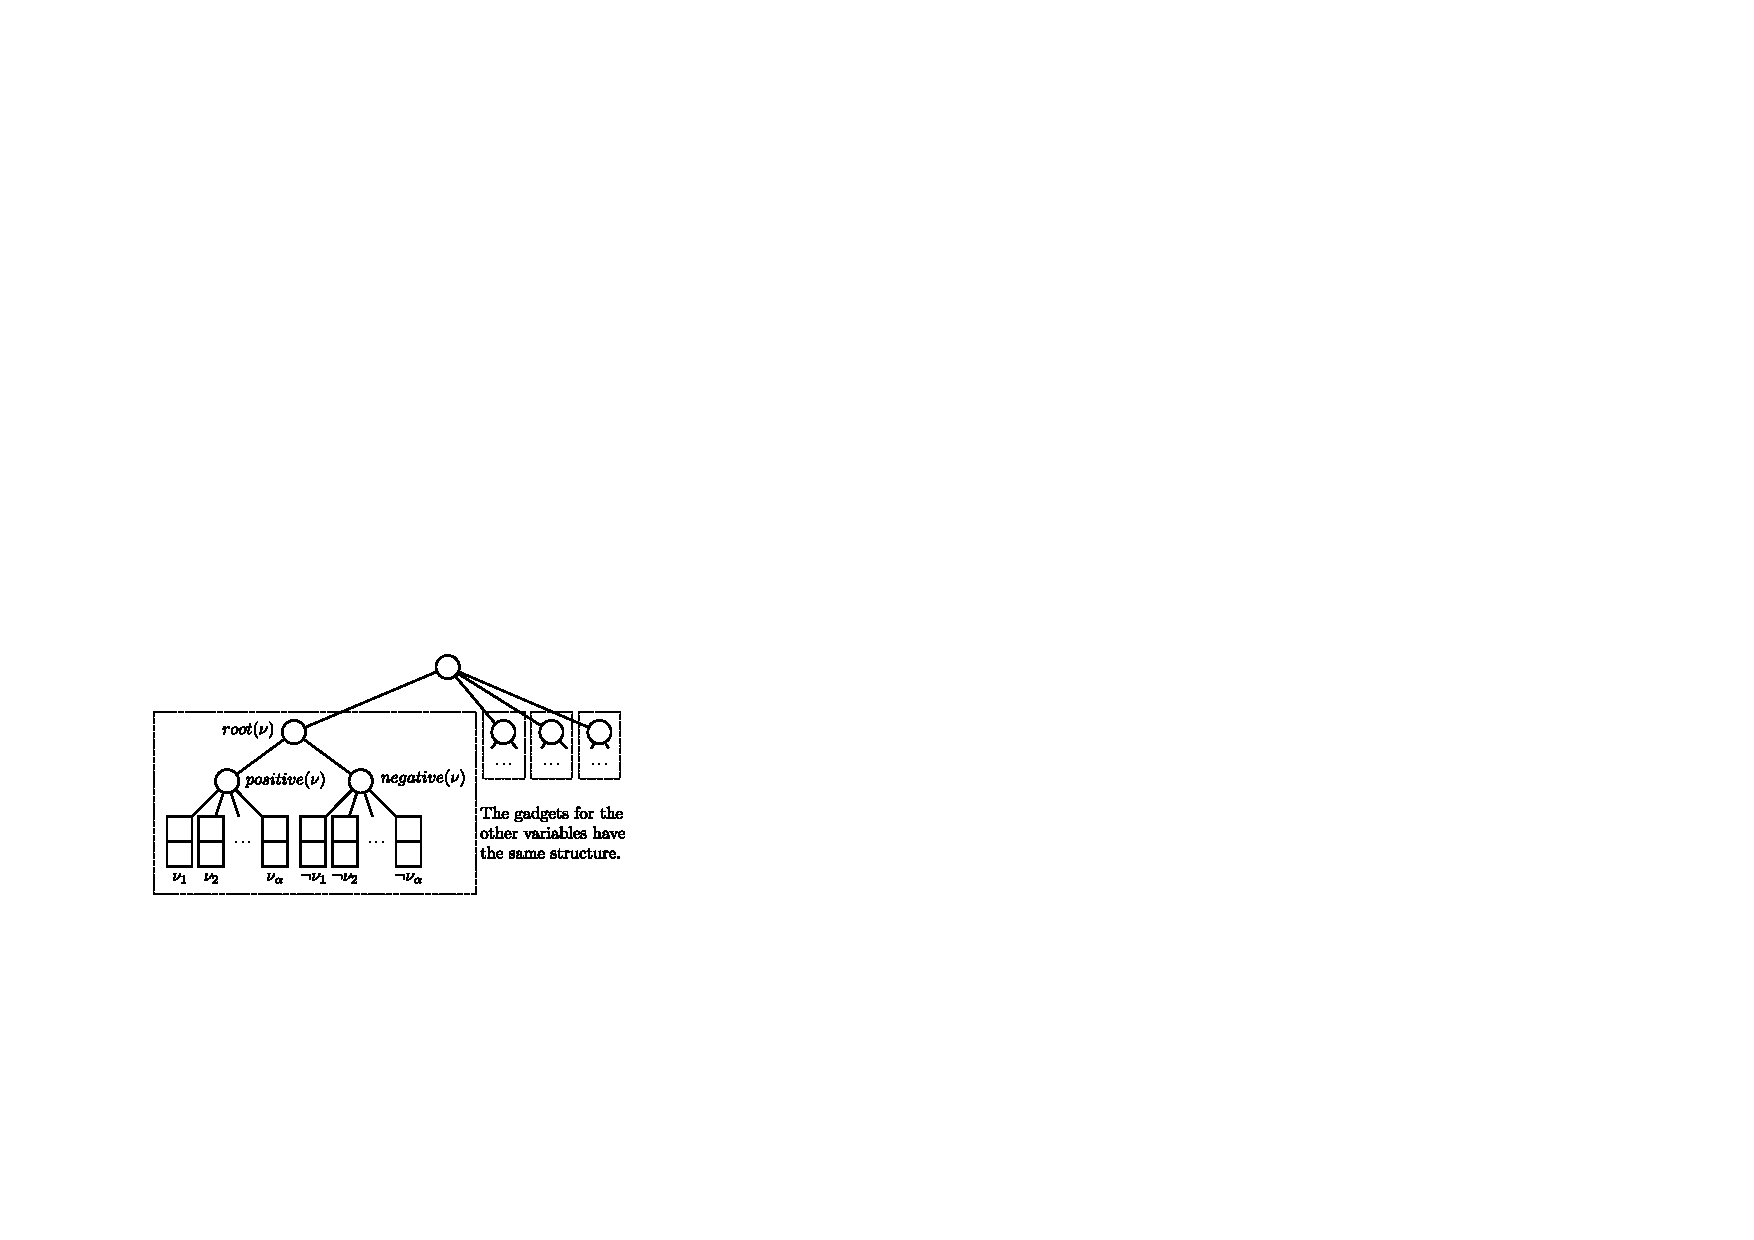
\includegraphics[width=\columnwidth]{figs/construction_3sat}
\caption{The construction of the gadget for $\nu$. If $\nu$ appears in the
first clause, a chunk $\achunk_1$, will be located at $\nu_1$. If $\neg \nu$
satisfies the last clause, $\neg
\nu_\alpha$ will host $\achunk_\alpha$.}
\label{fig:construction_3sat}
\end{figure}

\maciek{Following paragraph can be replaced with one sentence: ``We set bandwidth on uplink of each variable gadget to $\clauses \cdot (\clauses
\cdot \variables -
\clauses)$. We set other edges bandwidth to be unlimited.}

By default, we will set the available
bandwidth to be the
same everywhere, in every gadget; differences will be shown when we
will place chunks.
We set the following bandwidth capacities in the substrate. There are three
levels of edges in the substrate network $\Tree_{\Formula}$ given by formula
$\Formula$: \emph{top}, \emph{middle} and \emph{bottom}.
We do not consider any capacities at the \emph{bottom} and \emph{middle} levels.
At a top-level edge, we set the bandwidth to $\clauses \cdot (\clauses
\cdot \variables -
\clauses)$.



We set the number of nodes to $\Vms = \clauses \cdot \variables$.
Moreover, we define the inter-connect communication cost to be $1$,
and the access cost to be a sufficiently large constant $W$,
such that nodes must always be collocated with chunks. ($W$ in the order of
the threshold $\Thr$ is sufficient.)\maciek{Alternatively, we can set $W=1$ and restrict the transportation by setting bandwidth on uplink of every leaf.}

%(For a concrete value, see Appendix~\ref{ap:W}).

We set the number of chunk types to be equal to the number of clauses, $\tau =
\clauses$. To finish our construction, we place data chunks at
leaves, as follows: for the $i$-th clause we
construct as many replicas of chunk $\achunk_i$ as there are literals in the
clause. For each literal $\ell$ (of the form $\variab$ or $\neg \variab$) that satisfies clause $i$,
 we place
a replica of chunk $\achunk_i$ in the leaf labeled $\ell_i$.

\maciek{We want to say here how many VMs will be idle.}

We set the threshold $\Thr$ to:
% (\maciek{we might not want to introduce
%  those variable names, as those have no meaning here}):
$ \Thr = \variables \cdot ({\clauses  \choose 2} \cdot 2 +
\clauses \cdot (\clauses
\cdot \variables - \clauses))$.

\textbf{Proof of correctness of construction.}
We now show that our construction indeed
decides $\SAT$. We set the capacities such that in every gadget,
at most $\clauses$ nodes can be mapped, where $\clauses$
is the number of clauses of $\Formula$\maciek{Passive voice - consider rewrite.}
.
We can apply the Bandwidth Lemma (Lemma~\ref{lem:bandwidth-lemma}) as follows:
We interpret $a_i$ as the
number of nodes that are embedded in the $i$-th gadget, $\clauses$
as the number
of clauses, and $\variables$ as the number of variables.
The LHS of the inequality of Lemma~\ref{lem:bandwidth-lemma}
is a formula for the communication cost of nodes inside the $i$-th
gadget to nodes outside the gadget. The RHS of the inequality is the
bandwidth constraint for the gadget. This implies that
any feasible solution must embed exactly $\clauses$ nodes in every gadget.
(Recall that in our $\SAT$ instance, we have at least four variables.)

\begin{theorem}
The problem $\RS+\FP+\BW+\CC$ is NP-hard.
\end{theorem}
\begin{proof}
We will prove that formula $\Formula$ is satisfiable iff $\RS+\FP+\BW+\CC$ has
a solution of cost $\leq \Thr$.

($\Rightarrow$) Let us take any valuation $\Val$ that satisfies $\Formula$.
We will construct a solution to $\RS+\FP+\BW+\CC$ using $\Val$ in the following
way.
For each variable $\variab$ in $\Formula$, we embed $\clauses$ many nodes
at the  leaves of the gadget of $\variab$. We need to choose $\clauses$ out of
$2 \cdot \clauses$ leaves to embed nodes. If $\Val(\variab) = 1$, we embed
nodes at the leaves
of $\positive(\variab)$, else we embed all nodes at leaves $\negative(\variab)$.
The solution constructed this way has cost exactly
$\Thr$, because the nodes are evenly split among gadgets, and nodes are not
distributed across $\positive(\variab)$ and $\negative(\variab)$ subtrees.

We calculate the chunk-node matching $\mu$ by assigning every chunk to
the node which is collocated with the first chunk replica. This solution is feasible
(every chunk type is processed),
because the given valuation satisfied $\Phi$.

Now we will show that this solution has cost $\Thr$.
Due to the Bandwidth Lemma (Lemma~\ref{lem:bandwidth-lemma}),
we only have to consider the communication cost. We sum inner-gadget communication and communication among gadgets to get exactly $\Thr$.

($\Leftarrow$) Let us take any solution to $\RS+\FP+\BW$ constructed based on $\Formula$ of cost $\leq \Thr$.
We will construct a positive valuation $\Val$ by considering the nodes in
the solution to $\RS+\FP+\BW$.

We make the following observations. In every solution of cost
$\leq \Thr$, every gadget has exactly $\clauses$ many nodes
at its leaves. This is due to the Bandwidth Lemma (Lemma~\ref{lem:bandwidth-lemma}).
Also, inside
every gadget either all nodes are in the $\positive(\variab)$ subtree
of variable $\variab$, or in the $\negative(\variab)$ subtree. This is true
because the cost of a solution where at least one gadget has nodes
distributed across subtrees is
always greater than $\Thr$.

Now we can construct our valuation $\Val$, as follows
(for each variable $\variab$ in $\Formula$):
If $v_1$ hosts a node then $\Val(\variab) = 1$,
otherwise $\Val(\variab) = 0$.
%\carlo{Terminology deviates from above}

The valuation $\Val$ satisfies all clauses, and hence $\Formula$,
as the solution to $\RS+\FP+\BW$ covers all chunks. To see this,
consider the leaf which
hosts a node which is assigned to any given chunk (i.e.,
the leaf handling any given clause chunk);
it is a witness that the corresponding clause is satisfied.
\end{proof}

We conclude by observing that our construction leverages the fact that
the number of nodes may exceed the number of chunk types, e.g.,
for a clause $(x \vee y \vee z)$ in
$\Formula$, both $x$ and $y$ being true implies the
mapping of nodes on vertices labeled $x_1$ and $y_1$, and which contain the
same chunk $c_1$.


\subsection{Two replicas are hard
  ($\RS(2)+\FP+\CC+\BW$)}\label{ssec:two}

Our results so far indicate that dealing with replication can be challenging.
However, all our hardness proofs concerned scenarios with three replicas,
which raises the question whether the problems can be solved in polynomial time
with a replication factor of two only\maciek{Passive voice - consider rewrite.}
. (Similarly to, say, the $\ZSAT$ problem
which is tractable in contrast to $\TSAT$.)

In the following, we show that this is not the case: the problem remains
NP-hard, at least in the capacitated network.

The proof is by reduction from $\TSAT$. Given a formula $\Formula$ in
conjunctive normal form, consisting of $\clauses$ clauses and $\vars$ variables, we construct a problem instance and substrate tree
$T_{\Formula}$ using two types of gadgets: gadgets for variables and
gadgets for clauses. \emph{Nota bene:}
unlike in the previous proofs, for every clause we will create three chunk types instead of just one.

\includegraphics{figs/construction_2replica}

\carlo{TODO: caption of figure?}

\textbf{Construction.}
%\carlo{TODO: Describe construction of clause gadgets, and emphazise that we use
%the same construction as in Figure~\ref{fig:construction_3sat} for the variable
%gadgets. Introduce symbols for clauses, which can be transferred to the Figure.}
We build upon the construction for variable gadgets introduced (see also Figure~\ref{fig:construction_3sat}).

\begin{enumerate}
  \item \emph{Tree Construction}: In addition to the variable gadgets known from the
  previous construction, we introduce \emph{clause
    gadgets}. The clause gadget (illustrated in Figure~\ref{fig:clause-gadget})
    has two inner vertices:
    \emph{root}$(c)$, \emph{middle}$(c)$ and three leaves (we use the middle vertex mainly to
    preserve the balanced tree property). We connect leaves to the
    middle vertex, and the middle vertex to \emph{root}$(c)$. We attach the
    gadget to the tree by linking directly the global root to
    \emph{root}$(c)$. We construct our tree out of $\vars$ variable gadgets
    and $\clauses$ clause gadgets.
  \item \emph{Chunk Distribution:}
    We distribute two replicas of each of $\clauses \cdot 3$ chunk types among the servers as follows.
    First, similarly to the
previous proofs with three replicas, we put clause chunks into the variable
gadgets; however, now we place distinct chunks $c^{(1)}_i, c^{(2)}_i, c^{(3)}_i$
instead of three copies of the same chunk. Second, we place three
chunks that correspond to clauses in all three leaves of their clause
gadgets.  Thus, in total, $6 \cdot \clauses$ variable chunks are
mapped.  We will consider a setting where $\clauses \cdot \vars +
2\clauses$ nodes need to be mapped. Our intention is that in every
variable gadget, there will be $\clauses$ nodes, and in every clause
gadgets there will be two nodes.

  \item \emph{Bandwidth Constraints:}
    The available bandwidth of the top edge of the gadget of each variable $\variab$ is set to
$\capa(v) = 3  \cdot  3  \cdot  (3  \cdot  (\vars - 1) + 2  \cdot  \clauses)$.
The first factor is the distance in $\Tree$ which is 6 divided by 2 (as
we count each pair twice). The second factor is
the number of nodes to be placed in every variable gadget.
So the first term of the
sum is three times the number of outer variable gadgets,
and the second term is the
number of nodes in each of the $\clauses$ clause gadgets.
The available bandwidth for the top edge of each clause gadget is set to
$\capa(\clauses) = 3  \cdot  2  \cdot  (2  \cdot  (\clauses - 1) + 3  \cdot  \vars) $.
Notice that this construction uses two replicas of each chunk type:
one in the variable gadget and one in the clause gadget.

  \item \emph{Additional Properties:} We set the threshold in a
    similar fashion as in previous proofs. That is,
the threshold depends on the intra-clause communication cost (two hops),
inter-clause communication cost (4 hops),
  and the communication from variable gadgets to clause gadgets (4 hops) \maciek{This is wrong. Depending on 2 or 3 level clause gadget we need to modify one of number of hops)}. We
  set the number of nodes to be activated to $\clauses \cdot \vars + 2 \cdot
  \clauses$. We set the hosting capacity of each server to $1$, and set
  $\CostTrans = \Thr$ to disallow remote chunk access. We set $\CostCom = 1$.


 \end{enumerate}

\stefan{TODO Carlo: The construction is illustrated in Figure~\ref{fig:two}.}
\textbf{Proof of correctness.}
We first prove the following helper lemma.
\begin{lemma}
Every valid solution to $\FP+\RS(2)+\BW+\CC$
with cost at most $\Thr$ has the property that
there are exactly $\clauses$ nodes in each of the $\vars$ variable gadgets
and exactly two nodes in each of the $\clauses$ clause gadgets.
\end{lemma}
\begin{proof}
The claim is due to the bandwidth constraints.

\maciek{Following text is wrong, as it does not hold from respecting the threshold, rather that from extended bandwidth lemma and feasibility. I suggest removing the rest of the proof and only refer to ``Bandwidth lemmas'' section.}
We have to take into
consideration the following communication paths:
communication to clause gadgets and
communication to
other variable gadgets.
In every valid solution of cost at most $\Thr$, we have exactly
$\clauses$ nodes in each variable gadget and two nodes in each clause gadget.
\end{proof}


\begin{theorem}
$\FP+\RS(2)+\BW+\CC$ is NP-hard.
\end{theorem}
\begin{proof}
We show that $\FP+\RS(2)+\BW+\CC$ has a solution of cost $\leq
  \Thr$ if and only if $\Formula\in \TSAT$ is satisfiable.

($\Rightarrow$) If we have a positive valuation of $\Formula$, we fill variable gadgets with nodes like in
the proofs before. Then we fill $2 \cdot \clauses$ nodes as follows:
\begin{itemize}
\item If the first literal satisfies the clause, we map two nodes in the second and
third leaf of the corresponding clause gadget.
\item If the first literal does not satisfy the clause, we map two nodes to the first
and second leaf of the clause gadget.
\end{itemize}

We then assign chunks to nodes as follows:
\begin{itemize}
\item Chunk $\achunk_i^{(1)}$ is matched to the node which is located in a variable gadget; there
must be one, as the valuation satisfies the formula.
\item Chunks $\achunk_i^{(2)}$ and $\achunk_i^{(3)}$ are matched to nodes which
are
located in clause
gadgets
\end{itemize}

Thus, we have produced a feasible solution of cost $\Thr$.
($\Leftarrow$)
Let us take any solution $\Sol$ to $\RS(2)+\FP+\BW$ of cost $\leq \Thr$.
Then we can compute a positive valuation by setting each variable $\variab$
as follows:
$\Val(\variab)= 1$ iff there is a node at the first leaf on the positive side of the $\variab$ gadget in $\Sol$,
and $\Val(\variab)=0$ otherwise.

\maciek{We need to mention that the behavior of VMs inside variable gadget remain the same - VMs stick to one side (positive or negative). It is crucial property for the proof.}

%$\Val(\variab)$ =
%\begin{cases}
%\top & \mbox{iff there lies VM on first leaf on positive side of $\variab$ gadget in $\Sol$}\\
%\bot & \mbox{otherwise}
%\end{cases}

The theorem now follows from the following two additional lemmas.
\begin{lemma}
For every clause there exists a node in a variable gadget that processes one of
  three chunks that correspond to that clause.
\end{lemma}
\begin{proof}
 Each of the three chunks that correspond to each clause,
 is assigned a collocated node.
 At least one of those three nodes is not idle in a variable gadget;
otherwise, those two nodes in the clause gadgets would not suffice in
satisfying all chunk types.
\end{proof}

Observe that it might happen that in $\Sol$, two nodes in
clause variables are idle, and three nodes in variable gadgets are
processing those $3$ chunk types. In this case,
arbitrary nodes can be taken for the rest
of the proof\maciek{Passive voice - consider rewrite.}
.

\begin{lemma}
$\Val$ satisfies $\Formula$.
\end{lemma}
\begin{proof}
Let us consider the matching $M$ of $\Sol$, and let us consider an arbitrary clause of
$\Formula$ as well as its three chunk types: $\achunk_i^{(1)}, \achunk_i^{(2)}, \achunk_i^{(3)}$.
We will refer to the nodes corresponding to them
by $v_i^{(1)}, v_i^{(2)}, v_i^{(3)}$; two of them lie in clause gadgets.
Take the chunk type that was processed in variable
gadgets and look at where it was processed.
In our valuation $\Val$, we set the literal of the node leaf to
$1$; therefore the clause is satisfied.
\end{proof}

\maciek{We got lemmas formulated and proved inside the proof. IDK if we can do that. Also, we would like to conclude the 2 replica proof with a sentence or two (at least that it is NP-complete, not only NP-hard).}
\end{proof}

%\begin{comment}
%
%\subsection{Extended SAT bandwidth lemma proof}
%
%\maciek{Formulate lemma, and proof in the same way as the one in previous section}
%
%
%\begin{lemma}[Bandwidth Lemma]\label{lem:bandwidth-lemma}
%\maciek{this lemma might be expressed more clearly if we use two
%  sequences instead of one - now $a_1, \ldots, a_{\variables}$
%  correspond to number of VMs in variable gadgets and remaining of the
%  sequence corresponds to number of VMs in clause gadgets.}
%  Let $\clauses$ and $\variables > 4$ be two arbitrary positive integers. Let $a_1, a_2, \ldots,
%  a_{\variables+\clauses}$ be a sequence of integers which adds up to
%  $\clauses \cdot \variables + \clauses \cdot 2$. Also, for
%  each $i \leq \variables$ we have $a_i \leq 2 \cdot \clauses$
%  (\maciek{variable gadget capacity}). Also,
%  for each $i >\variables$ we have $a_i \leq 3$ (\maciek{clause gadget capacity}). Then it holds that if
%  $$ \forall_{i\leq\variables}:~~ a_i \cdot (\clauses \cdot \variables
%  + 2\cdot \clauses- a_i) \leq \clauses \cdot (\clauses \cdot \variables -
%  \clauses + 2 \cdot \clauses), $$
%and
%$$ \forall_{i>\variables}:~~ a_i \cdot (\clauses \cdot \variables + 2 \cdot \clauses - a_i) \leq 2 \cdot (\clauses \cdot \variables -
%  2 \cdot \clauses - 2), $$
%
%\noindent  then for each $i\leq \variables$: $a_i = \clauses$ and for
%each $i>\variables$: $a_i = 2$.
%\end{lemma}
%
%\maciek{proof will be painful and we should skip on showing that,
%  pointing into the previous proof. Even if we did this proof, nobody
%  would read that. I can do it though.}
%\end{comment}
\section{The Bandwidth Lemmas}

\maciek{Those are lemmas helpful in proving that in every bandwidth-feasible solution of cost $\leq \Thr$ there is certain amount of empty gadgets and certain amount of half-full gadgets. Bandwidth lemma is helpful in reduction from 3SAT to RS, and extended bandwidth lemma is helpful in reduction from 3SAT to RS(2). TODO: reference those lemmas in both proofs in the appendix!}
  
\begin{lemma}[Bandwidth Lemma]\label{lem:bandwidth-lemma}
  Let $\clauses$ and $\variables > 4$ be two arbitrary positive integers. Let $a_1, a_2, \ldots,
  a_{\variables}$ be a sequence of $\variables$ integers which adds up to $\clauses \cdot \variables$. Also, for
  each $i$ we have $a_i \leq 2 \cdot \clauses$. Then it holds that if
  $$ \forall_i:~~ a_i \cdot (\clauses \cdot \variables - a_i) \leq \clauses \cdot (\clauses \cdot \variables -
  \clauses), $$
\noindent  then for each $i$: $a_i = \clauses$.
\end{lemma}
\begin{proof}
  \maciek{(By contradiction) Let us assume...}
For the sake of contradiction, let us assume that there exists an index $k$ such that
$a_k \neq \clauses$. Then we can distinguish between two cases:
either $a_k<\clauses$ or
$a_k>\clauses$.

\textbf{Case $a_k<\clauses$:} If there exists a $k$ with $a_k<\clauses$,
due to the fact that the sequence adds up to $\clauses \cdot \variables$,
there must also exist a $k'$ such that $a_{k'}<\clauses$ (by a simple
pigeon hole principle). Thus, this case can
also be reduced to the second case (Case $a_k>\clauses$) proved
next.

\textbf{Case $a_k>\clauses$:} Since it also holds that $a_k < 2\clauses$,
$a_k$ must be of the form $\clauses + x$ for $x \in [1, \ldots, \clauses]$.
Let us consider the (bandwidth) inequality:
$$ (\clauses + x) \cdot (\clauses \cdot \variables - \clauses - x) \leq \clauses \cdot (\clauses \cdot \variables - x) $$

This can be transformed to\maciek{Passive voice - consider rewrite.}
:

$$ 0 \leq x(x - (\clauses \cdot (\variables - 2))) $$

The equation holds for $x \leq 0$ or $x \geq \clauses \cdot (\variables - 2)$,
and no
positive $x \leq \clauses$ can satisfy this inequality for $\variables > 4$. Contradiction.
\end{proof}
\begin{lemma}[Extended Bandwidth Lemma]\label{lem:bandwidth-lemma}
%\maciek{this lemma might be expressed more clearly if we use two
%  sequences instead of one - now $a_1, \ldots, a_{\variables}$
%  correspond to number of VMs in variable gadgets and remaining of the
%  sequence corresponds to number of VMs in clause gadgets.}
  Let $\clauses$ and $\variables > 4$ be two arbitrary positive integers. Let $a_1, a_2, \ldots,
  a_{\clauses}$ and $b_1, b_2, \ldots,
  b_{\variables}$ be two sequences of integers (numbers of VMs in clause and in variable gadgets). Sum of all elements in $a$ and $b$ adds up to
  $\clauses \cdot \variables + \clauses \cdot 2$ (number of VMs). Also
  we have $a_i \leq 2 \cdot \clauses$
  (variable gadget VM hosting capacity -- equal to number of leaves),
  and $b_i \leq 3$ (clause gadget VM hosting capacity). If uplink of variable gadget does not exceed bandwidth constraints
  $$ \forall_{i\leq\variables}:~~ b_i \cdot (\clauses \cdot \variables
  + 2\cdot \clauses- b_i) \leq \clauses \cdot (\clauses \cdot \variables -
  \clauses + 2 \cdot \clauses), $$
and uplink of clause gadget does not exceed bandwidth constraints
$$ \forall_{i\leq\clauses}:~~ a_i \cdot (\clauses \cdot \variables + 2 \cdot \clauses - a_i) \leq 2 \cdot (\clauses \cdot \variables -
  2 \cdot \clauses - 2), $$

\noindent  then for each $i\leq \variables$: $b_i = \clauses$ and for
each $i\leq\clauses$: $a_i = 2$ (we have expected number of VMs in variable and clause gadgets).
\end{lemma}



\end{appendix}



\end{document}
